\documentclass[]{elsarticle} %review=doublespace preprint=single 5p=2 column
%%% Begin My package additions %%%%%%%%%%%%%%%%%%%

\usepackage[hyphens]{url}

  \journal{An awesome journal} % Sets Journal name

\usepackage{graphicx}
%%%%%%%%%%%%%%%% end my additions to header

\usepackage[T1]{fontenc}
\usepackage{lmodern}
\usepackage{amssymb,amsmath}
% TODO: Currently lineno needs to be loaded after amsmath because of conflict
% https://github.com/latex-lineno/lineno/issues/5
\usepackage{lineno} % add
  \linenumbers % turns line numbering on
\usepackage{ifxetex,ifluatex}
\usepackage{fixltx2e} % provides \textsubscript
% use upquote if available, for straight quotes in verbatim environments
\IfFileExists{upquote.sty}{\usepackage{upquote}}{}
\ifnum 0\ifxetex 1\fi\ifluatex 1\fi=0 % if pdftex
  \usepackage[utf8]{inputenc}
\else % if luatex or xelatex
  \usepackage{fontspec}
  \ifxetex
    \usepackage{xltxtra,xunicode}
  \fi
  \defaultfontfeatures{Mapping=tex-text,Scale=MatchLowercase}
  \newcommand{\euro}{€}
\fi
% use microtype if available
\IfFileExists{microtype.sty}{\usepackage{microtype}}{}
\usepackage[]{natbib}
\bibliographystyle{elsarticle-harv}

\ifxetex
  \usepackage[setpagesize=false, % page size defined by xetex
              unicode=false, % unicode breaks when used with xetex
              xetex]{hyperref}
\else
  \usepackage[unicode=true]{hyperref}
\fi
\hypersetup{breaklinks=true,
            bookmarks=true,
            pdfauthor={},
            pdftitle={A historical analysis of the evolution of active travel behaviour in Canada},
            colorlinks=false,
            urlcolor=blue,
            linkcolor=magenta,
            pdfborder={0 0 0}}

\setcounter{secnumdepth}{5}
% Pandoc toggle for numbering sections (defaults to be off)


% tightlist command for lists without linebreak
\providecommand{\tightlist}{%
  \setlength{\itemsep}{0pt}\setlength{\parskip}{0pt}}




\usepackage{booktabs}
\usepackage{longtable}
\usepackage{array}
\usepackage{multirow}
\usepackage{wrapfig}
\usepackage{float}
\usepackage{colortbl}
\usepackage{pdflscape}
\usepackage{tabu}
\usepackage{threeparttable}
\usepackage{threeparttablex}
\usepackage[normalem]{ulem}
\usepackage{makecell}
\usepackage{xcolor}



\begin{document}


\begin{frontmatter}

  \title{A historical analysis of the evolution of active travel
behaviour in Canada}
    \author[Some Institute of Technology]{Alice Anonymous%
  \corref{cor1}%
  \fnref{1}}
   \ead{alice@example.com} 
    \author[Some Institute of Technology]{Bob Security%
  %
  \fnref{1}}
   \ead{bob@example.com} 
    \author[Some Institute of Technology]{Cat Memes%
  %
  }
   \ead{cat@example.com} 
      \affiliation[Some Institute of Technology]{
    organization={Big Wig University},addressline={1 main
street},city={Gotham},postcode={123456},state={State},country={United
States},}
    \cortext[cor1]{Corresponding author}
    \fntext[1]{These authors contributed equally to this work.}
  
  \begin{abstract}
  Impedance functions are used to represent travel behaviour due to
  their potential to capture traveler responses to geographic distance
  between origins and destinations. Focusing our analysis on active
  transportation modes in Canadian metropolitan regions, this study has
  as objectives to provide an historical overview of active mobility in
  terms of main origins, destinations and travel time of walking and
  cycling trips, and to identify appropriate impedance functions for
  active transportation modes considering a wide range of destinations
  and time periods. To achieve these objectives, this paper analyzed
  more than cases of 12,000 active transportation episodes, that
  represented more than 12 million episodes, from the Canadian General
  Social Survey (GSS) from 1992 to 2015. This study confirmed that for
  walking trips, typical travel times remained constant at 10 minutes
  since 2005, while for cycling trips, typical travel times fluctuated,
  declining from 20 minutes in 1992 to 10 minutes in 2010 before
  increasing to 20 minutes in 2015. For walking trips, findings indicate
  that `Home' continues to be the main hub, either as an origin or
  destination. For cycling trips, the combination of `Home' and `Work or
  school' accounted for most of the trips. Additionally, we fitted 64
  impedance functions for twelve destinations and over 20 years. The
  results indicate that none of the parameterized functions were
  exponential, suggesting that the impedance functions commonly used in
  active accessibility studies may not accurately capture travel
  behavior, especially for very short trips, giving shorter trips a
  higher probability of being made. The estimated impedance functions
  can be employed in active accessibility analysis to help to reduce the
  dependence on private vehicles and promote healthier, more sustainable
  travel behaviour.
  \end{abstract}
    \begin{keyword}
    Active mobility \sep Walking \sep Cycling \sep Impedance
function \sep 
    Temporal evolution
  \end{keyword}
  
 \end{frontmatter}

\section{Introduction}\label{introduction}

The idea that travel behaviour can be influenced by city form has
attracted growing interest in urban and transportation planning. Cities
intent to encourage residents to adopt more sustainable modes of
transportation, such as walking, cycling, and public transit, by
developing environments that offer diverse transportation alternatives
while simultaneaously improving accessibility - defined as the of
reaching destinations and opportunities \citep{iacono2008access}. Active
transportation modes, including walking and cycling, play a important
role in enhancing and promoting urban sustainability
\citep{hino2014built, lamiquiz2015effects}, making them central to urban
mobility research and policy-making
\citep{handy1993regional, clifton2001evaluating, frank2001built, krizek2005perspectives, sallis2004active, vandenbulcke2009mapping, wu2019measuring}.
Walking and cycling accessibility are closely related, jointly
contributing to the concept of ``active accessibility'' or
``non-motorized accessibility''. when incorporated into urban and
transportation planning, they help to reduce the dependence on private
vehicles and promote healthier, more sustainable travel behaviour among
residents.

There are two main components when measuring accessibility: the location
and power of attraction of urban opportunities (trip benefit), and the
barrier in travel from the origin to the destination (trip cost). A way
for measuring the cost of travel when calculating accessibility is using
impedance functions, a methods that is receiving attention from
transportation planning scholars, urban geography, and sustainable
development
\citep{frank2005linking, krizek2005perspectives, currie2010quantifying, iacono2010, yang2012walking, millward2013active, nassir2016utility, saghapour2017measuring, wu2019measuring}.
The impedance functions have different forms and all of them serve as a
tool to understand the travel behaviour, since they work as measure of
the willingness to travel a certain distance to achieve a desired
destination, where a service or an opportunity is located
\citep{taylor1975distance, fotheringham1981spatial, kwan1998space, eldridge1991warped, luoma1993threshold, papa2012gravity, yang2012walking, millward2013active, vale2017influence}.
In this concept, areas with higher accessibility are those characterized
by a lower impedance when traveling to desirable destinations. In
relation to active accessibility, increasing the distance between two
points generally implies in a probability decrease of that trip being
done by walking or biking
\citep{hansen1959accessibility, pirie1979measuring, handy1997measuring, geurs2001accessibility, bhat2002development, church2003measuring, kwan2003recent, geurs2004, levinson2005access, cascetta2013new}.
However, more information about the willingness of some individuals to
walk or cycle greater distance is needed, as well as more data on how
distance affects the type and feasibility of the activity, destinations
desirability, and the characteristics of those embarking on the trip in
different situations. In this context, investigate the evolution and
dynamics of impedance function over time becomes important, since they
are easily impacted by changes in the transportation network or in urban
spatial configurations \citep{iacono2008access, iacono2010}. Luoma,
Mikkonen, and Palomaki \citeyearpar{luoma1993threshold} evidenced a
decreasing in the distance decay parameter over time in the province of
Vaasa, Finland, attributing this trend to improvements and maturation of
the transportation system \citep{luoma1993threshold}. A few years later,
Mikkonen and Luoma \citeyearpar{mikkonen1999parameters} argued that this
difference was mainly caused by the establishment of new big retail
store units, elucidating the factors behind these temporal patterns in
the gravity models patterns \citep{mikkonen1999parameters}.

Since the beginning applications of the gravity-accessibility models, a
range of impedance functions have been applied to describe the
distribution of walking and cycling trips, wether for general or
specific purposes
\citep{iacono2008access, iacono2010, larsen2010beyond, yang2012walking, millward2013active, vale2017influence, li2020approach}.
Selecting an appropriate impedance function can be challenging and
results in a diverse range of cost decay functions that are employed as
impedance functions in accessibility measures, including \emph{threshold
functions} (e.g., binary Step Function and multiple Step Function) and
\emph{smooth cost decay functions} (e.g., log-normal, normal, gamma, and
exponential function)
\citep{de2009exponential, reggiani2011accessibility, osth2016new, itf2017linking}.
The variety of functions relies in how scholars approach the influence
of distance, with negative exponential distance-decay functions are
commonly used in assessing non-motorized accessibility, capturing the
willingness of individuals to walk or cycle to destinations
\citep{handy1997measuring, geurs2001accessibility, iacono2010, vega2012using, millward2013active, vale2017influence, li2020approach}.

The merit of negative exponential function is due to its ability to
assign decreasing influences to more remote opportunities, giving a more
accurate estimate for shorter trips
\citep{iacono2010, kanafani1983transportation, fotheringham1989spatial}.
However, in addition to determine the form of the impedance function,
scholars also need to specify the variable used to measure impedance,
which can be either time, distance, monetary cost, a combination these
last variables or even a generalized cost concept. Among these options,
the choice between time and distance as the impedance has been found to
be most used based on previous studies
\citep{iacono2010, hull2012accessibility, sun2012measuring, lowry2012using, vasconcelos2012evaluation},
with distance being more adopted in non-motorized applications since
extracting accurate travel times from existing network models can be
challenging
\citep{handy1997measuring, iacono2010, yang2012walking, arranz2019measuring}.
Additionally, estimate impedance function to active transportation modes
requires appropriate travel survey data that captures pedestrian and
cycle behaviour, resulting in researchers recurring to retrospective
questionnaires to assess subjective aspects such as the frequency and
duration of walking and cycling activities. Notably, regional household
travel surveys that include trips made by non-motorized modes have been
employed for this purpose \citep{iacono2010, millward2013active}. In
opposition to these specific surveys, some data sets provides a
nationwide perspective, including travel for different purposes and
detailing the trip with valuable information, named episodes, regarding
the origins, destinations, and time-based lengths. Besides this type of
data can provides a deeper comprehension about the active transportation
behaviour, only few studies have examined travel behaviour nationally.

Having presented this context, this paper poses the questions: What is
the typical travel time for active transportation modes (walking and
cycling) in Canadian metropolitan regions, considering various
destinations and years? Which impedance functions best represent active
transportation travel behavior? To answer the research questions, this
study has as two main objectives: first, to provide an overview of the
active transportation in terms of main origins, destinations, and travel
time; and second, to identify appropriate impedance functions for active
transportation modes for different destinations and time periods in
Canadian metropolitan areas. To do achieve both objectives, we utilize
data provided by the \texttt{ActiveCA} R package
\citep{dossantos2024ActiveCA}, an open data product in the form of an R
data package with information about active travel in Canada. This data
product is based on Public Use Microdata Files of Statistics Canada's
General Social Survey (GSS) program with a focus on the Time Use Survey
cycles. To build this package, the authors extracted all walking and
cycling episodes and their corresponding episode weights for GSS cycles,
Cycles 7 (1992), 12 (1998), 19 (2005), 24 (2010), and 29 (2015),
spanning a period of almost thirty years. Origins and destinations were
categorized, enabling the investigation of active travel for broad
destination categories and purposes.

We recognize that non-work travel encompasses a range of trip purposes
and diverse traveler behaviors, which makes impedance functions
essential analytical tools for studying non-work accessibility. Grengs
\citeyearpar{grengs2015nonwork} emphasizes the importance of elaborating
distinct functions for each travel purpose, a principle that guides this
analysis. Our investigation covers a variety of trip purposes, ranging
from commutes to homes, workplaces, or educational institutions to
social visits, outdoor activities, business trips, shopping, cultural
outings to libraries, museums, or theaters, dining out, and engaging in
religious practices. Our research aims to enhance the current knowledge
about active travel behaviour and provide empirical data about frequency
and duration of typical pedestrian and cycling trips for different
purposes, by applying the methodology on a nationally representative
samples of Canadian residents. Lastly, this analysis seeks to contribute
to the ongoing conversation on active transportation, highlighting its
role in influencing transportation plans to a more sustainable
alternative.

\section{Background}\label{background}

Accessibility is the main benefit provided by the transportation system
\citep{pereira2017}, being understood as the potential to access
spatially distributed opportunities
\citep{hansen1959accessibility, páez2012}. When computing accessibility
measure, is necessary take into account the challenges associated with
this access to different locations and opportunities. Usually, the
effect of travel costs is expressed by ``impedance functions'', also
called ``distance decay functions''
\citep{hansen1959accessibility, koenig1980indicators, fotheringham1981spatial}.

Overall, impedance functions are derived from estimates based on
distributions of sample data that reflect variations in the willingness
of individuals to travel different distances to reach opportunities
\citep{hsiao1997use, zhao2003forecasting, iacono2010, li2020approach}.
Their main objective is to describe the decrease in the intensity of
interaction as the cost of travel between locations increases. The cost
of travel is usually measured in terms of the distance between the
places of origin and destination, or in terms of the time spent reaching
the destination from the point of origin.

In fact, distant facilities are less likely to be used compared to
closer ones
\citep{hansen1959accessibility, koenig1980indicators, fotheringham1981spatial, skov2001estimation}.
Thus, the ``distance decay'' effect suggests that adding a unit of
distance to a long trip is less significant than adding a unit to a
shorter trip \citep{carrothers1956historical}, since the farther
location already has a lower probability of access for the person
willing to travel.

Examining the impedance functions across different modes of transport
and destinations is a good way to understand the travel behavior
associated with each mode, while also helping to examine allegations
about travel behavior. Current interest in creating ``livable''
communities often relies on broad assumptions about individuals'
willingness to walk or bike to different destinations. For example, it
is commonly assumed that people are generally willing to walk up to a
quarter mile to access most places \citep{untermann1984accommodating}.
Similarly, the recent ``15-minute city'' concept proposes that the
majority of daily necessities should be accessible by walking or cycling
within 15 minutes \citep{moreno2021}.

\subsection{Impedance functions in accessibility
measures}\label{impedance-functions-in-accessibility-measures}

Since the research of Hansen \citeyearpar{hansen1959accessibility},
different categories of accessibility measures have been developed, such
as indicators based on actives, infrastructure, individuals and
utilities \citep{geurs2004, páez2012}. The family of gravity-based
accessibility have been widely used in active modes
\citep{miller2005place}. Many gravity-based accessibility measures
derive from the work of Hansen \citeyearpar{hansen1959accessibility},
represented in (Equation \ref{eq:accessibility-equation}), in which an
impedance function weights opportunities:

\begin{equation}
A_{i} = \sum_{j=1}^J O_j .f(c_{ij})
\label{eq:accessibility-equation}
\end{equation}

The accessibility score \(A_{i}\) at each origin \(i\) is obtained by
summing up the opportunities \(O\) available at destination \(j\), where
\(i\) and \(j\) are sets of spatial units in a region. However, the
number of opportunities in each destination is gradually discounted as
travel costs become higher and the the rate at which this weight
decreases is determined by a decay function. \(f(c_{ij})\) represents
the impedance during the trip from origin \(i\) to destination \(j\) and
\(c_{ij}\) reflects the generalized travel cost, potentially
encompassing factors such as time, distance and effort. In this way, the
impedance function \(f(c_{ij})\) allows the accessibility analyst to
define a measure of travel behavior with precision: the relationship
between the ``population'' at an origin and where they normally want to
or can go to reach ``opportunities'' at destinations. The definition of
the impedance function \(f(c_{ij})\) is very important from this
perspective.

Another type of family of accessibility measures are \emph{cumulative
opportunity} metrics, commonly referred to as isochronous indices. The
binary function Equation (\ref{eq:cumulative-equation}) forms the basis
of the cumulative opportunities maeasure approach. This function
determine accessibility by summing up the number of opportunities
available within a specific limiar of travel time or distance from a
reference point, without discounting the potential of the trip in
relation to the associated cost. They use a rectangular function,
categorizing the trip as ``acceptable'' within certain limits and
``unacceptable'' beyond them. One of the main complexities of these
metrics is deciding what the appropriate limiar point is. This decision
may be based on the prevailing mobility patterns of the population or
may reflect established norms, conventions or informed projections of
the researcher. Note that the cumulative opportunity measure can be
understood as a special case of a gravity-based measure in which the
weight of each opportunity is defined by a binary function, rather than
a gradually decaying function \citep{pereira2023}.

\begin{equation}
C_{ij} =
\begin{cases}
  1 & \text{if } c_{ij} \le x \\
  0 & otherwise
\end{cases}
\label{eq:cumulative-equation}
\end{equation}

Among the various mathematical forms that can represent impedance
functions, the negative exponential function is the dominant choice in
accessibility research
\citep{meyer1984urban, gutierrez1996european, kwan1998space, apparicio2008comparing, iacono2008access, iacono2010, larsen2010beyond, millward2013active}.
Its high adoption can be attributed mainly to its ability to give
greater weight to nearby opportunities, and greater weight to distant
opportunities - a highly relevant characteristic for active modes of
transportation, such as walking and cycling. When Hansen
\citeyearpar{hansen1959accessibility} introduced their accessibility
measure, the author applied and indicated the use of exponential
distributions \((e ^ {-\beta x})\) as the impedance function. After
this, several other studies
\citep{fotheringham1989spatial, de2009exponential, iacono2010, signorino2011gravity, prins2014many}
use the negative exponential function after comparison with empirical
trip distribution data.

Researchers can adopt other forms of impedance functions when
calculating the distance decay effect in accessibility analysis. One of
these options is to adopt a probability density function (PDF)
\citep{soukhov2024}. Using a PDF, \(f()\) can be interpreted as the
probability density of a trip occurring for each value of travel cost
\(c_{ij}\). If a graph of the PDF (y-axis) is plotted against the travel
cost \(c_{ij}\) (x-axis), the probability of a trip occurring between a
given range of \(c_{ij}\) is the area under the curve. In this case, the
total area under the PDF curve always sums to 1, meaning that there is
100\% probability that the trip will occur between the minimum and
maximum \(c_{ij}\).

Dunn et al. \citeyearpar{dunn2023} presented a set of distributions that
serve as PDFs. From their survey, we selected some options for \(f()\)
commonly used in accessibility research and their impact on the number
of opportunities (the sum of opportunities) at specific travel costs
\(c_{ij}\), namely: uniform, negative exponential, gamma, normal, and
lognormal distributions.

\begin{itemize}
\tightlist
\item
  \textbf{Uniform distribution}
\end{itemize}

The uniform distribution or rectangular PDF looks very similar to the
binary function, since it only returns one of two values, but ensure
that area under the curve for the range of \(c_{ij}\) is 1. The uniform
distribution PDF is shown in (Equation \ref{eq:uniform-equation}).

\begin{equation}
f(c_{ij})^{uniform} =
\begin{cases}
  \frac{1}{c_{max} - c_{min}} & \text{for } c_{min} \le c_{ij} \le c_{max} \\
  0 & \text{otherwise}
\end{cases}
\label{eq:uniform-equation}
\end{equation}

The parameters to be calculated are \(c_{max}\) and \(c_{min}\), which
represent the maximum and minimum travel costs that describe the
observed or assumed willingness to reach destinations. In this
distribution, all values within the interval are equally likely, and all
values outside the interval have probability 0, assuming that the
population's potential to interact with these opportunities is zero.
Usually, \(c_{min}\) has value 0.

\begin{itemize}
\tightlist
\item
  \textbf{Exponential distribution}
\end{itemize}

The exponential distribution PDF equation is given by Equation
(\ref{eq:exponential-equation}). This model suggests that impedance
decreases exponentially with increasing cost \((c_{ij})\). The parameter
\(\beta\) represents the decay rate, with higher values indicating a
faster decrease in accessibility with increasing cost. As already
mentioned, this function is widely used due to its simplicity and
ability to model the rapid drop-off in accessibility over distance.

\begin{equation}
f(c_{ij}) = e^{-\beta c_{ij}} \text{ with } c_{ij} \ge 0
\label{eq:exponential-equation}
\end{equation}

\begin{itemize}
\tightlist
\item
  \textbf{Gamma distribution}
\end{itemize}

The gamma distribution PDF equation is presented by the Equation
\ref{eq:gamma-equation}.

\begin{equation}
f(c_{ij}) = 
   \begin{cases}
\frac{1}{\sigma^\alpha\Gamma(\alpha)} c_{ij}^{\alpha-1} e^{\frac{-c_{ij}}{\sigma}} & \text{if } 0 \leq c_{ij} <      \infty  \text{ and } \alpha, \sigma > 0 \\ 0 & \text{otherwise}
   \end{cases}
\label{eq:gamma-equation}
\end{equation}

Where \(\Gamma(\alpha)\) is the gamma function to be estimated. In this
case, the probability is typically low at low cost, higher at medium
cost, and low again at high cost. The higher the \(\sigma\) (scale rate)
parameter, the higher the probability that the majority of trips will be
in the low cost range. So at low values of the \(\sigma\) (scale rate)
parameter, the same probability is spread over a wider range of travel
costs. For the \(\alpha\) (shape) parameter, the higher the value, the
higher the probability density of trips with a higher average cost
\citep{soukhov2024}.

\begin{itemize}
\tightlist
\item
  \textbf{Lognormal distribution}
\end{itemize}

The normal distribution, also often called the Gaussian distribution, is
suitable when the travel cost is found to be distributed normally. The
normal distribution has the PDF form displayed in Equation
(\ref{eq:normal-equation}).

\begin{equation}
f(c_{ij}) = \frac{1}{\sqrt{2\pi} \sigma c_{ij}} e^{-\frac{(\ln c_{ij} - \mu)^2}{2\sigma^2}}
\label{eq:normal-equation}
\end{equation}

In this equation, \(\mu\) and \(\sigma\) are the mean and standard
deviation of the distribution and need to be estimated together to
control the shape of the normal curve. In this distribution, about 68\%
of the observations will fall within 1 standard deviation of the mean,
about 95\% will fall within 2 standard deviations, and about 99.7\% will
fall within 3 standard deviations of the mean. In this case, the values
close to the mean will have the highest probability.

\begin{itemize}
\tightlist
\item
  \textbf{Lognormal distribution}
\end{itemize}

In many cases, the logarithm of the travel cost is found to be
distributed normally. The lognormal distribution has the PDF form
displayed in Equation (\ref{eq:lognormal-equation}).

\begin{equation}
f(c_{ij}) = \frac{1}{\sqrt{2\pi} \sigma c_{ij}} e^{-\frac{(\ln c_{ij} - \mu)^2}{2\sigma^2}}
\label{eq:lognormal-equation}
\end{equation}

It this equation, \(\mu\) and \(\sigma\) are the mean and standard
deviation of the logarithm, and need to be estimated for together
control the shape of the log-normal curve. Similar to the gamma
function, the probability is typically low at low cost, higher at medium
cost, and low again at high cost.

As the complexity of the PDF increases, so does the flexibility to
explain travel behaviour. However, the estimation of the impedance
function parameters needs to be calibrated if the accessibility
estimates are to be representative of people's travel behaviour. This
requires additional travel behaviour data to be used in the calibration
process. In our case, we will use the \texttt{ActiveCA} package
\citep{dossantos2024ActiveCA} to obtain the impedance functions, as the
package contains ready-to-use data from GSS cycles.

\subsection{The GSS survey}\label{the-gss-survey}

The GSS provides a comprehensive cross-sectional snapshot of the
Canadian population through telephone surveys established in 1985
\citep{statisticscanada2022}. The survey coverage area includes both
metropolitan and non-metropolitan regions, ensuring a diverse and
representative sample of the Canadian population. Specifically, the
seven provinces and three territories of Canada were divided into
distinct geographic strata for sampling purposes. Many Census
Metropolitan Areas (CMAs), such as St.~John's, Halifax, Saint John,
Montreal, Quebec City, Toronto, Ottawa, Hamilton, Winnipeg, Regina,
Saskatoon, Calgary, Edmonton, and Vancouver, were treated as separate
strata. Additional strata were formed by grouping other CMAs within
Quebec, Ontario, and British Columbia, and by categorizing non-CMA areas
within each province into their own strata.

These surveys encompass an array of socio-demographic inquiries combined
with questions concentrating on specific core themes, such as health,
time use, and aspects like social support and aging. One of the standout
features of the GSS is its recurring ``time use'' cycle
\citep{statisticscanada2022}, which concentrates in the daily activities
of Canadians. This cycle captures the amount of time individuals
allocate to various tasks and the sequence, location, and concurrent
activities, offering a wide view of Canadians' daily lives. The
questions within this cycle have been adapted and refined over the years
to reflect the changing dynamics of daily life, ensuring that the data
remains pertinent and contemporary.

\section{Materials and Methods}\label{materials-and-methods}

To investigate the historical active travel behavior in Canada, we
analyzed five GSS Time Use cycles: Cycles 7 (1992), 12 (1998), 19
(2005), 24 (2010), 29 (2015) and 37 (2022). We excluded Cycle 2 (1986)
from our analysis because this survey did not specify whether the
respondent lived in a metropolitan area and did not present cycling as a
mode of transportation option, although this cycle is notable for having
been the first national random sample to examine Canadian time-use
patterns. This paper is a direct application of the ready-to-use data
set provided by the \texttt{ActiveCA} data package
\citeyearpar{dossantos2024ActiveCA}, which is based on the Main and
Episode files from the GSS Public Use Microdata Files. The Main file
contains questionnaire responses and associated data from participants,
while the Episode files provided detailed information about every
activity episode reported by the respondents.

The methodology involves two main steps, each designed to achieve one of
our primary objectives. The first step employs descriptive analysis of
active transportation episodes to identify typical travel times across
destinations and years, comparing their temporal evolution and
identifying differences in active transportation episodes through
statistical tests. The second step calculates and analyzes impedance
functions for each combination of cycle, destination, and active travel
mode.

To facilitate collaboration and further analysis, we updated the
\texttt{ActiveCA} R Package to include the methodology to obtain
impedance functions from the raw data files (GSS surveys). Additionally,
we created this paper using literate programming in which the R markdown
code to fully reproduce this article is available on our GitHub
repository \emph{(include after the review)}, in line with the best
practices of spatial data science \citep{arribas-bel2021, páez2021}.
These contributions improve our understanding of active travel behaviour
in Canada and provide a basis for future research and policy-making.

\subsection{Analyzing active travel
episodes}\label{analyzing-active-travel-episodes}

For each selected cycle of the GSS surveys, we reviewed the episode
files to identify cases with activities listed as walking or cycling,
selecting the locations immediately before and after the mobility
episode. With this process, we were able to identify the origin and the
destination of the active travel episode. We labeled the code variables
with their appropriate descriptions, identifying the transportation
mode, activity/reason of the travel, as well the province and urban
classification of the respondent's residency (if the respondent lives in
a CMA or in a Census Agglomerations).

Additionally, it was necessary to guarantee the data consistency across
the surveys, since they have employed a variety of variable coding
schemes. The range of activities and destinations considered in the
surveys changed from 1992 to 2022. In 1992, there were only three
options of origin/destination location available to the respondent:
their home, other's home and work or study. In its turn, the most recent
survey (2022) counts with twelve possible destination, including sport
area (sports centre, field or arena), restaurant (including bar and
club), health clinics (medical, dental or other health clinic), grocery
stores (including other types of stores and malls) and more. In order to
achieve uniformity, the activity categories from 2005, 2010, 2015, and
2022 were synchronised, and a similar process was employed for those
from 1992 and 1998. For the preceding years (1992, and 1998), the trip
origins and destinations were classified as ``Home,'' ``Other's home,''
and ``Work or school.'' In the subsequent years (2005, 2010, 2015, and
2022), these categories were expanded to include ``Business,''
``Restaurant'' ``Place of worship,'' ``Grocery store''
``Neighbourhood,'' ``Outdoors,'' ``Cultural venues'' (such as library,
museum and theatre), and ``Sport area.'' This evolution in data
collection reflects a growing understanding of the complex nature of
urban mobility and the diverse purposes that motivate walking and
cycling trips, providing a comprehensive foundation for analyzing
distance decay and its implications for urban planning and sustainable
transportation strategies.

Statistical analysis was used to characterize active travel episodes
using cross-tabulations and graphs. Summary statistics and visualization
techniques, including median values as a measure of typical value and
boxplots, were employed to describe active travel across years,
destinations, and transportation modes. To assess the statistical
significance of potential temporal differences in the empirical episode
data set for each destination, we applied the Kruskal-Wallis test. This
test was chosen because it does not assume a normal distribution for the
data, an important consideration since we made no assumptions about the
distribution of the empirical data. The identification of impedance
functions serves as the step that captures the distributional
characteristics of the empirical values. The Kruskal-Wallis test
evaluates differences in the medians of the empirical data.

\subsection{Analyzing the population with active travel
records}\label{analyzing-the-population-with-active-travel-records}

After assessing the active travel episodes, we analyzed the population
with records of active travel for each year of the analysis. First, we
identified the population with and without at least one active travel
episode, considering both modes (walking and cycling). After that, for
the active population, we examined how active episodes were distributed
across the available destinations for each survey year. Finalizing the
population analysis, we measured the number of active trips per person
for each year, considering both the active and general population.

\subsection{Estimating impedance function
parameters}\label{estimating-impedance-function-parameters}

We applied the \texttt{fitdistrplus} package
\citep{delignette2015fitdistrplus} to calculate the best PDF for every
destination, mode of transportation and survey year, between the
options: uniform, negative exponential, gamma, normal, and lognormal
distributions. In order to calculate the impedance functions, two
filters were applied in the GSS data set. The first is that we excluded
all trips with travel times higher than 100 minutes (1.5 hours). An
exploratory data analysis showed that, taking into account all the
walking and cycling episodes (19,166 in total), less than 0.73\% of the
episodes have a trip duration higher than this limit. When considering
the weights of this episodes, travel times higher than 100 minutes
represented 0.93\% of the episodes.

It was also possible to know that trips with a duration higher than 100
minutes are mainly composed of hiking and camping episodes. The second
filter was realized to select only the population living in a larger
urban population centre. We decided to apply this restriction because
the travel behaviour of residents of CMA and CA areas tends to be very
different from those outside these large urban centres in terms of
active travel.

\section{Results and discusion}\label{results-and-discusion}

\subsection{Descriptive analysis}\label{descriptive-analysis}

\subsubsection{Walking and cycling
episodes}\label{walking-and-cycling-episodes}

After applying the filters to the GSS surveys, we obtained a total of
19,166 lines with active travel episodes. However, GSS surveys apply a
probability sampling methodology, in which each episode or person
selected in the sample represents several other episodes or persons not
in the sample. The number of episodes and persons represented by a
episode or person is determined by the weight or weighting factor.
Because of this, every estimates of the number of episodes or persons
need to be calculated applying the corresponding weighting factors.

Considering the weights - and from this point onward, all counts
estimates presented in this paper account for them - the 19,166 episodes
represent a total of 28,066,620 episodes. Table
\ref{tab:episodes-count-percentages} contains the weighted number of
episodes about walking and cycling trips between 1992 and 2022, obtained
from the GSS cycles. The year 2010 is the year with the most episodes,
with 7,116,460 episodes (representing 25.36\% of the total). The year
2010 is followed by 2005 with 6,152,778, representing approximately
21.92\% of all active travel episodes; followed by 2015 (5,921,772
episodes, 21.1\% of the total), 2022 (5,335,510 episodes, 19.01\% of the
total), 1998 1,773,061 episodes, (6.32\% of the total), and 1992, with
only 1,767,041 episodes, representing 6.3\% of the total.

When analyzing the two active transportation modes, walking episodes
account for 91.56\%, while the remaining 8.44\% are cycling episodes.
The most recent survey (2022) showed that bicycle trips accounted for
almost 10\% of active travel episodes, reinforcing an increasing trend
in the participation since 2005 - the year that marked the lowest
representation, as opposed to 1992, when bicycle episodes marked the
highest participation in all years (13\%).

\begingroup\fontsize{8}{10}\selectfont

\begin{longtable}[t]{lcccccccccccccc}
\caption{\label{tab:bulding table-01}\label{tab:episodes-count-percentages}Weighted number of episodes identified in each active transportation mode by year}\\
\toprule
\multicolumn{1}{c}{ } & \multicolumn{2}{c}{1992} & \multicolumn{2}{c}{1998} & \multicolumn{2}{c}{2005} & \multicolumn{2}{c}{2010} & \multicolumn{2}{c}{2015} & \multicolumn{2}{c}{2022} & \multicolumn{2}{c}{Total} \\
\cmidrule(l{3pt}r{3pt}){2-3} \cmidrule(l{3pt}r{3pt}){4-5} \cmidrule(l{3pt}r{3pt}){6-7} \cmidrule(l{3pt}r{3pt}){8-9} \cmidrule(l{3pt}r{3pt}){10-11} \cmidrule(l{3pt}r{3pt}){12-13} \cmidrule(l{3pt}r{3pt}){14-15}
Mode &  & (\%) &  & (\%) &  & (\%) &  & (\%) &  & (\%) &  & (\%) &  & (\%)\\
\midrule
Cycling & 230316.9 & 13.03 & 156123.1 & 8.81 & 472839.5 & 7.68 & 559295.6 & 7.86 & 475626.6 & 8.03 & 474128.9 & 8.89 & 2368331 & 8.44\\
Walking & 1536723.8 & 86.97 & 1616937.8 & 91.19 & 5679938.1 & 92.32 & 6557164.6 & 92.14 & 5446144.9 & 91.97 & 4861380.6 & 91.11 & 25698290 & 91.56\\
Total & 1767040.7 & 6.30 & 1773060.9 & 6.32 & 6152777.6 & 21.92 & 7116460.2 & 25.36 & 5921771.5 & 21.10 & 5335509.5 & 19.01 & 28066620 & 100.00\\
\bottomrule
\end{longtable}
\endgroup{}

Tables \ref{tab:table-02} presents statistic on travel time by active
transportation mode. The maximum time spent on walking trips varied
between 90 and 100 minutes across the years. It is important to remember
that trips with duration greater than 100 minutes were excluded from the
analysis. The mean walking time also varies, starting at 20 minutes in
1992, dropping to 12 minutes between 1992 to 2005, and increasing again
to 13 minutes in 2010, to 16 minutes in 2015, and to 18 minutes in 2022.
However, it is known that the mean is a statistic that is highly
influenced by extreme values. For this reason, we analyze the median
travel time, as it is more representative of the typical travel time.
The median time spent walking was 10 minutes in 1992, dropped to 5
minutes in 1998, remained constant at 10 minutes from 2005 to 2015, and
increased to the highest level in 2022, to 15 minutes.

\begingroup\fontsize{8}{10}\selectfont

\begin{longtable}[t]{>{}llcccccc}
\caption{\label{tab:table-02}\label{tab:table-02}Descriptive statistics for episodes with active transport records}\\
\toprule
\multicolumn{2}{c}{ } & \multicolumn{6}{c}{Year} \\
\cmidrule(l{3pt}r{3pt}){3-8}
Mode & Statistic & 1992 & 1998 & 2005 & 2010 & 2015 & 2022\\
\midrule
 & Maximum & 90 & 100 & 100 & 90 & 95 & 90\\
\nopagebreak
 & Mean & 20 & 12 & 12 & 13 & 16 & 18\\
\nopagebreak
 & Median & 10 & 5 & 10 & 10 & 10 & 15\\
\nopagebreak
 & Minimum & 5 & 1 & 1 & 1 & 5 & 5\\
\nopagebreak
\multirow[t]{-5}{*}{\raggedright\arraybackslash \textbf{Walking}} & Standard deviation & 19 & 13 & 12 & 13 & 13 & 15\\
\cmidrule{1-8}\pagebreak[0]
 & Maximum & 90 & 80 & 95 & 100 & 90 & 60\\
\nopagebreak
 & Mean & 21 & 28 & 20 & 18 & 24 & 30\\
\nopagebreak
 & Median & 20 & 25 & 15 & 10 & 20 & 30\\
\nopagebreak
 & Minimum & 5 & 2 & 1 & 2 & 5 & 5\\
\nopagebreak
\multirow[t]{-5}{*}{\raggedright\arraybackslash \textbf{Cycling}} & Standard deviation & 20 & 19 & 16 & 16 & 15 & 14\\
\bottomrule
\end{longtable}
\endgroup{}

For cycling trips, the maximum travel time ranges from 60 to 100
minutes. Until 2022, maximum travel times had a similar pattern to
walking trips, but the new survey showed that the maximum travel time
for cycling trips was the lowest when considering all years for both
modes (walking and cycling). The average cycling travel time varied
considerably, ranging from 18 minutes in 2010 to 30 minutes in 2022.
When we analyze the median travel time, we see that the typical cycling
travel time also fluctuated between the periods, starting at 20 minutes
in 1992 and peaking at 30 minutes in 2022. As was also the case with the
walking travel times, these results show a trend of increasing for
cycling trip duration throughout the years. The analysis of travel time
statistics alone does not fully explain the reasons behind these
fluctuations in travel time over the years. However, it is likely that
these variations reflect changes in bicycle technology or cyclist
behavior.

Figure \ref{fig:figure-destmodeyearperc} shows the percentage of each
destination by year and by mode of transport. For all the years
analyzed, `Home' is the most common travel destination, regardless of
whether the mode of transport considered is walking or cycling, with
levels above 40\%. After that, `Work or school' appears as the second
most common destination, especially for journeys by bicycle, with a peak
of almost 36\% of trips by bicycle in 1998, followed by a high drop to
23\% in 2005. Along with the two destinations already mentioned,
`Other's home' is the only other destination present in the GSS surveys
since 1992. This last destination seems to be a destination with a
higher share when it comes to walking trips, but for both modes of
transportation it seems that respondents are going less and less to
other people's homes - a fact that can be explained by new communication
technologies, in which a person does not need to visit another person's
home to keep in touch with them.

\begin{figure}
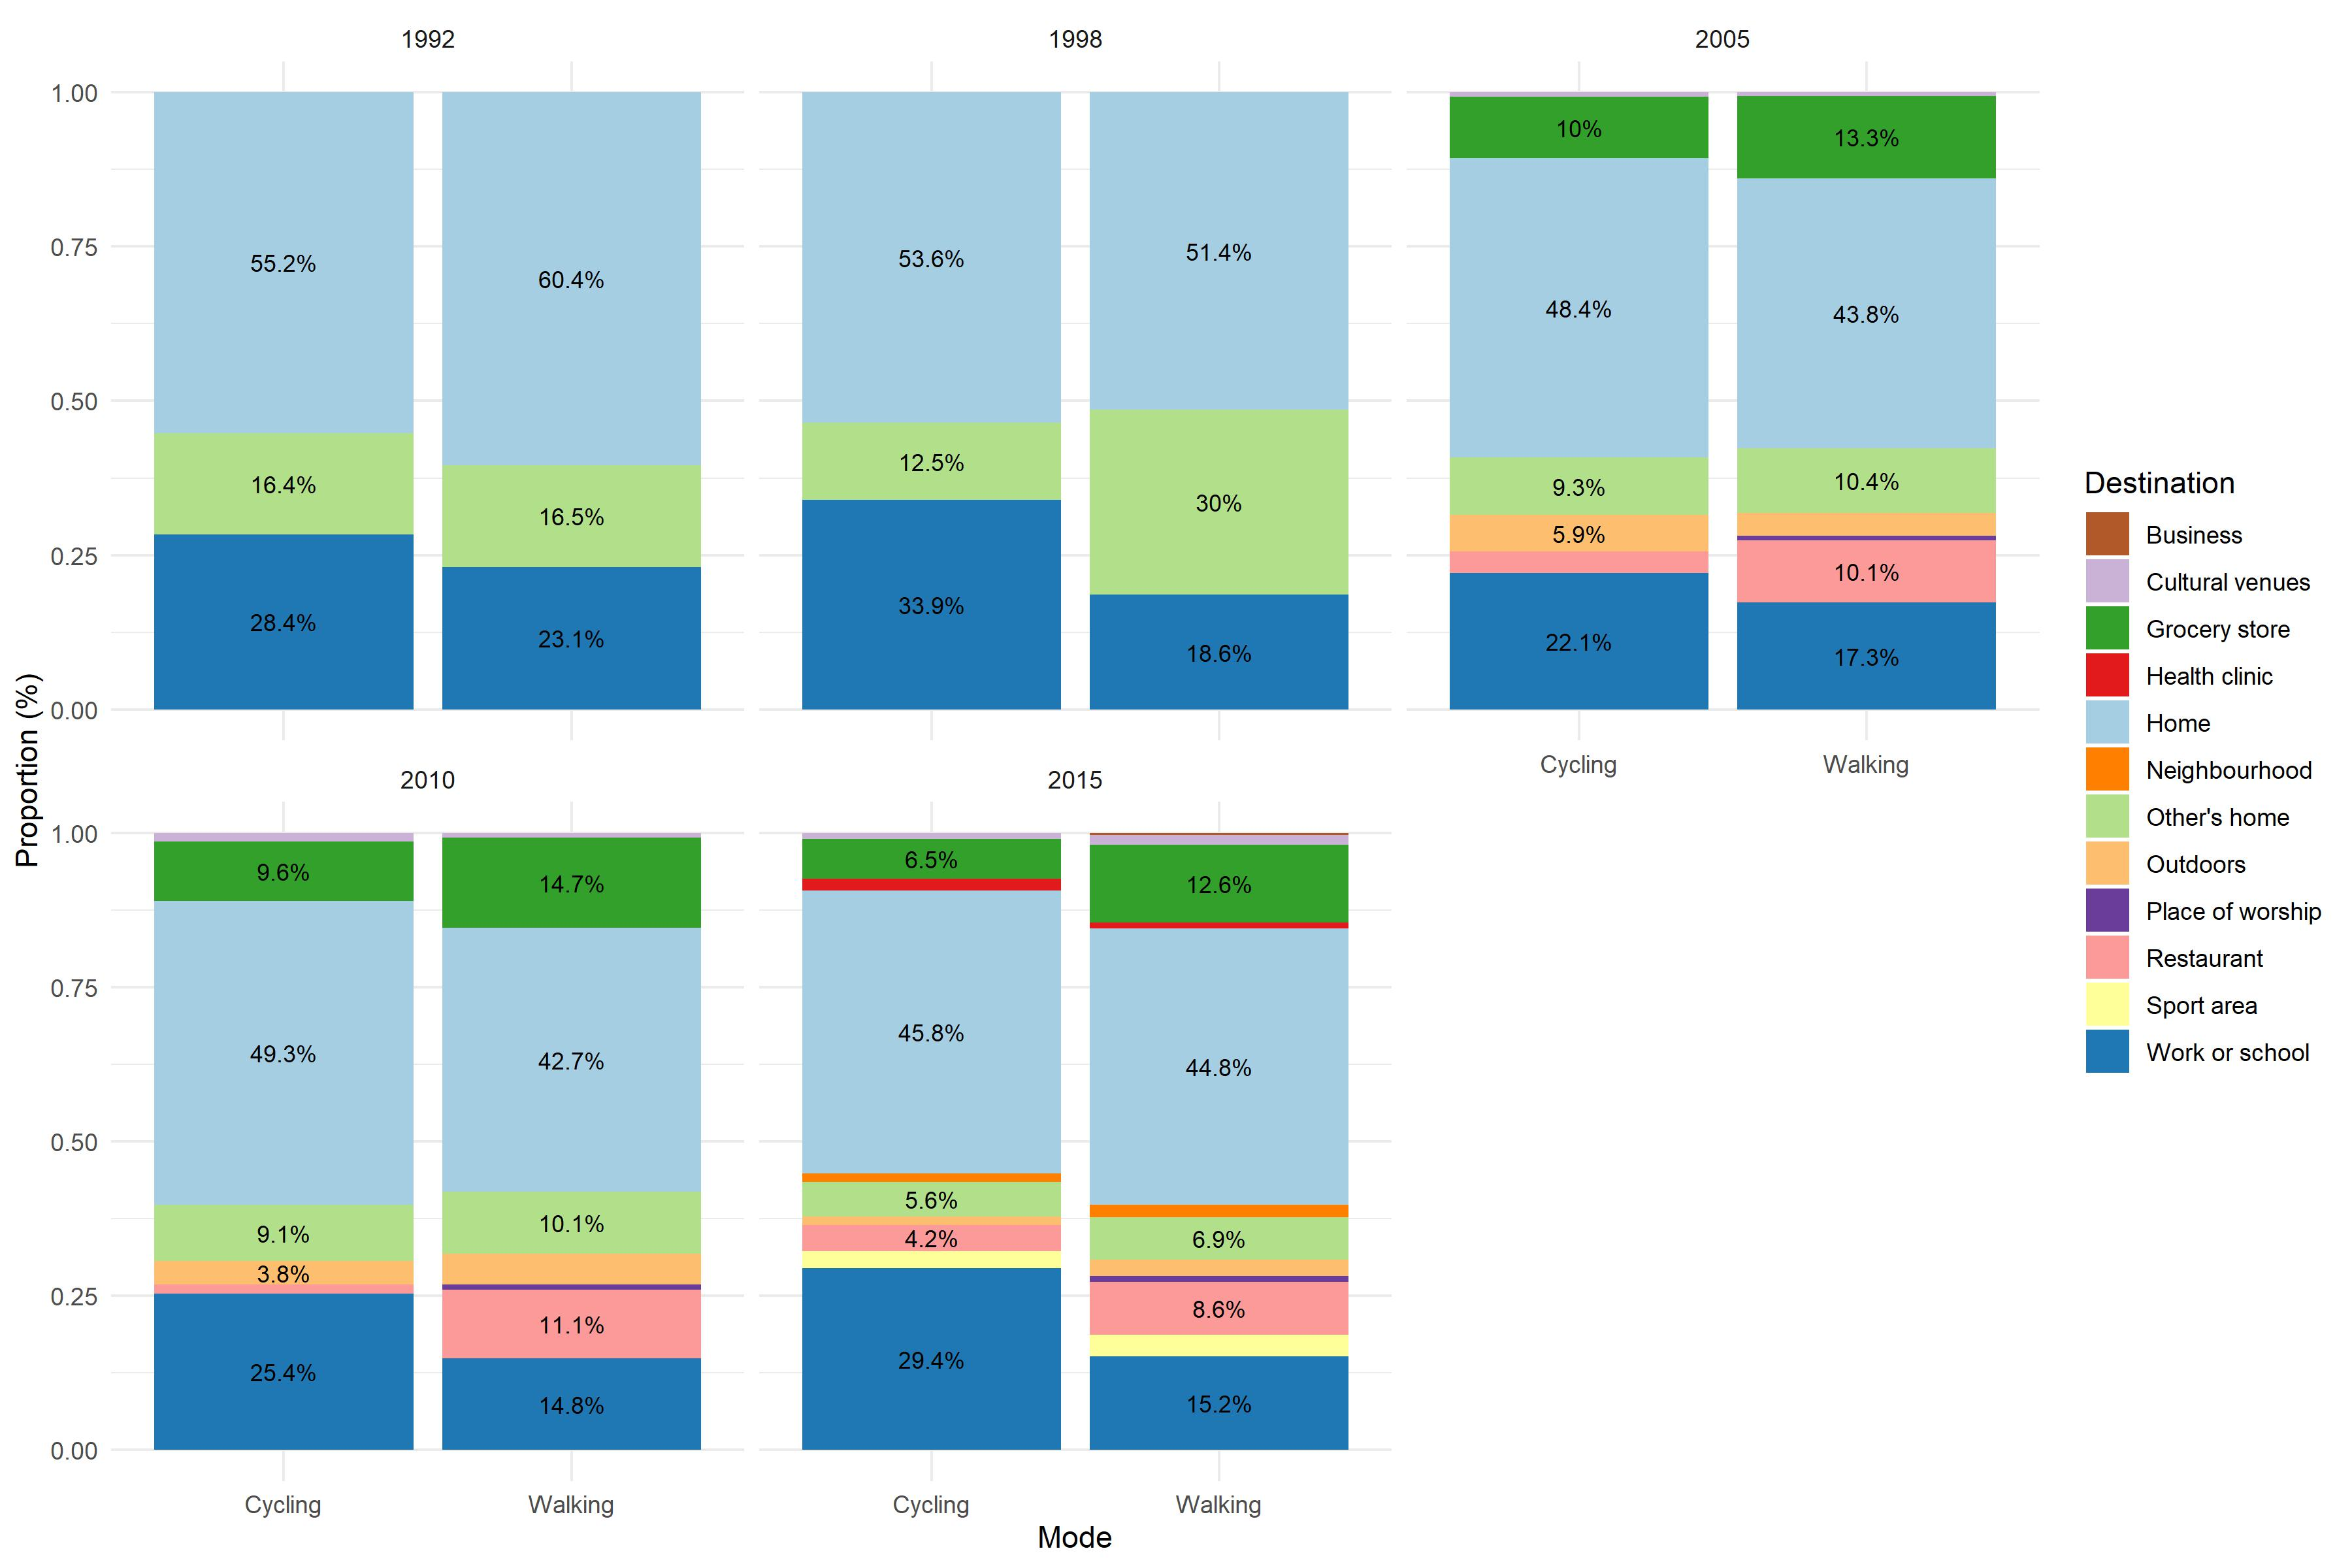
\includegraphics[width=1\linewidth]{figures/destination_percentual} \caption{Percentage of walking and cycling trips categorized by destination and year}\label{fig:figure-destmodeyearperc}
\end{figure}

After 2005, the expansion of the destination highlights some new popular
locations. For example, `Grocery store' appears as the third most chosen
destination, varying from almost 10\% in 2005 to 14.3\% in 2022 for
cycling trips and from 12\% to 12.6\% for walking trips. When
considering walking trips, `Restaurants' appears as another well chosen
destination and, in the case of cycling trips, `Outdoors' appears as a
well chosen destination.

Figure \ref{fig:figure-boxplot} presents box plots showing the
distribution of travel times for active transport modes over the years,
categorized by destination. During the period studied, the typical
duration of walking trips was consistently shorter than that of cycling
trips. While we can compare the temporal evolution of travel times, some
destinations appear only in the two most recent surveys, such as
``Neighborhood,'' ``Health clinic,'' ``Sports area,'' and ``Business.''
The first three showed a constant walking travel time of 10 minutes in
both surveys, while the travel time to ``Business'' increased from 10 to
15 minutes. For cycling trips, ``Business'' recorded no trips, while
``Neighborhood'' had a typical travel time of 30 minutes in 2015 but no
records for 2022. ``Health clinic'' showed a constant cycling travel
time of 15 minutes, and ``Sports area'' doubled its typical duration,
from 15 to 30 minutes.

\begin{figure}

\includegraphics[width=1\linewidth]{figures/destination_boxplots} \caption{Percentage of walking trips categorized by origin and destination}\label{fig:figure-boxplot}
\end{figure}

For the other destinations, starting with walking trips, we note a trend
of increasing travel times for almost all destinations, with an increase
observed at least in the most recent survey (2022). ``Restaurants'' and
``Outdoors'' both increased from 5 minutes in 2005 to 10 minutes in
2022; ``Other's home'' rose to 10 minutes in 2022 after remaining at 5
minutes since 1992; ``Place of worship'' increased from 10 minutes in
2005 to 20 minutes in 2022; and ``Cultural venues'' rose from 10 minutes
in 2005 and 2010 to 20 minutes in 2022. The three most popular types of
destinations - ``Home,'' ``Work or school,'' and ``Grocery store'' - had
an increase to 15 minutes after decades of stabilization at 10 minutes.
In general, while ``Place of worship'' and ``Cultural venues'' displayed
the highest median travel times of 20 minutes, the overall median
walking time cutoff across all surveys appears to be 10 minutes, with
most trips occurring below this threshold. In this case, no destination
shows a decrease in typical (median) travel time.

For cycling trips, only ``Cultural venues'' did not show an increase in
typical travel time when comparing 2022 to the previous years. In this
case, the travel time dropped from 25 minutes in 2010 to 15 minutes in
2015, although it remained higher than the 2005 value (10 minutes), and
no trips were recorded in the most recent survey (2022). ``Other's
home'' is the other destination with no cycling records for the 2022
survey. An increasing trend in travel times is evident for destinations
such as ``Grocery store'' (rising from 10 to 60 minutes between 2005 and
2022) and ``Restaurant'' (rising to 30 minutes in 2022).

Other destinations seem to follow a similar pattern of increasing travel
time, where higher values were recorded in earlier survey cycles,
dropped over time, and then rose again in the most recent surveys. This
is the case for ``Home,'' which reached its highest typical travel time
of 25 minutes after dropping to 10 minutes in 2010. It is also worth
mentioning ``Work or school,'' which had a typical cycling travel time
of 15 minutes in 1992, peaked at 30 minutes in 1998, dropped back to 15
minutes in 2005 and 2010, and then increased to 25 minutes in 2022. In
this case, no destination shows a decrease in typical (median) travel
time.

Figures \ref{fig:walking-heatmap} and \ref{fig:cycling-heatmap} show
walking and cycling trips from 1992 to 2022 through heat maps. These
maps use color gradients to represent the percentage of trips between
origins and destinations, with darker colors indicating higher
percentages and lighter colors representing less frequent routes. In
1992, walking trips with `Home' as both the origin and destination made
up the majority, accounting for almost 31\% of all walking trips. These
trips often involved leisure activities, like short walks or dog
walking. Following this, trips from `Home' to `Work or school' comprised
18\% of walking trips. Overall, `Home' is the principal hub, either as
an origin or destination, with only 7\% of trips not involving `Home.'
By 1998, more than half of walking trips were between `Home' and
`Other's home,' with `Home' to `Other's home' and `Other's home' to
`Home' each representing 26\% of trips. During this year, `Home' to
`Home' accounted for only 10\% of trips. In 2005, trips with origins or
destinations involving `Home' and `Work or school' remained as the most
common, but the introduction of new destinations led to a more dispersed
trip distribution. Together, these two combinations accounted for 25\%
of all trips. In 2010, trips between `Home' and `Work or school'
continued as the most common type, representing 18\% of trips, tied with
trips from `Grocery store' to `Home' (9\%).In 2015, the highest
proportion of trips were from ``Home'' to ``Work or school'' (12\%) and
vice versa (11\%). Trips from ``Home'' to ``Home'' accounted for 8\% of
trips, and the ``Grocery store'' became a notable destination for trips
originating from ``Home'' (8\%) - patterns that were reinforced, as
shown in the 2022 survey. In the most recent survey, the most common
trip was from ``Home'' to ``Work or school'' (17\%), followed by the
return trip from ``Work or school'' to ``Home'' (13\%). After that,
trips between ``Home'' and the ``Grocery store'' accounted for 20\% when
both directions are combined.

\begin{figure}
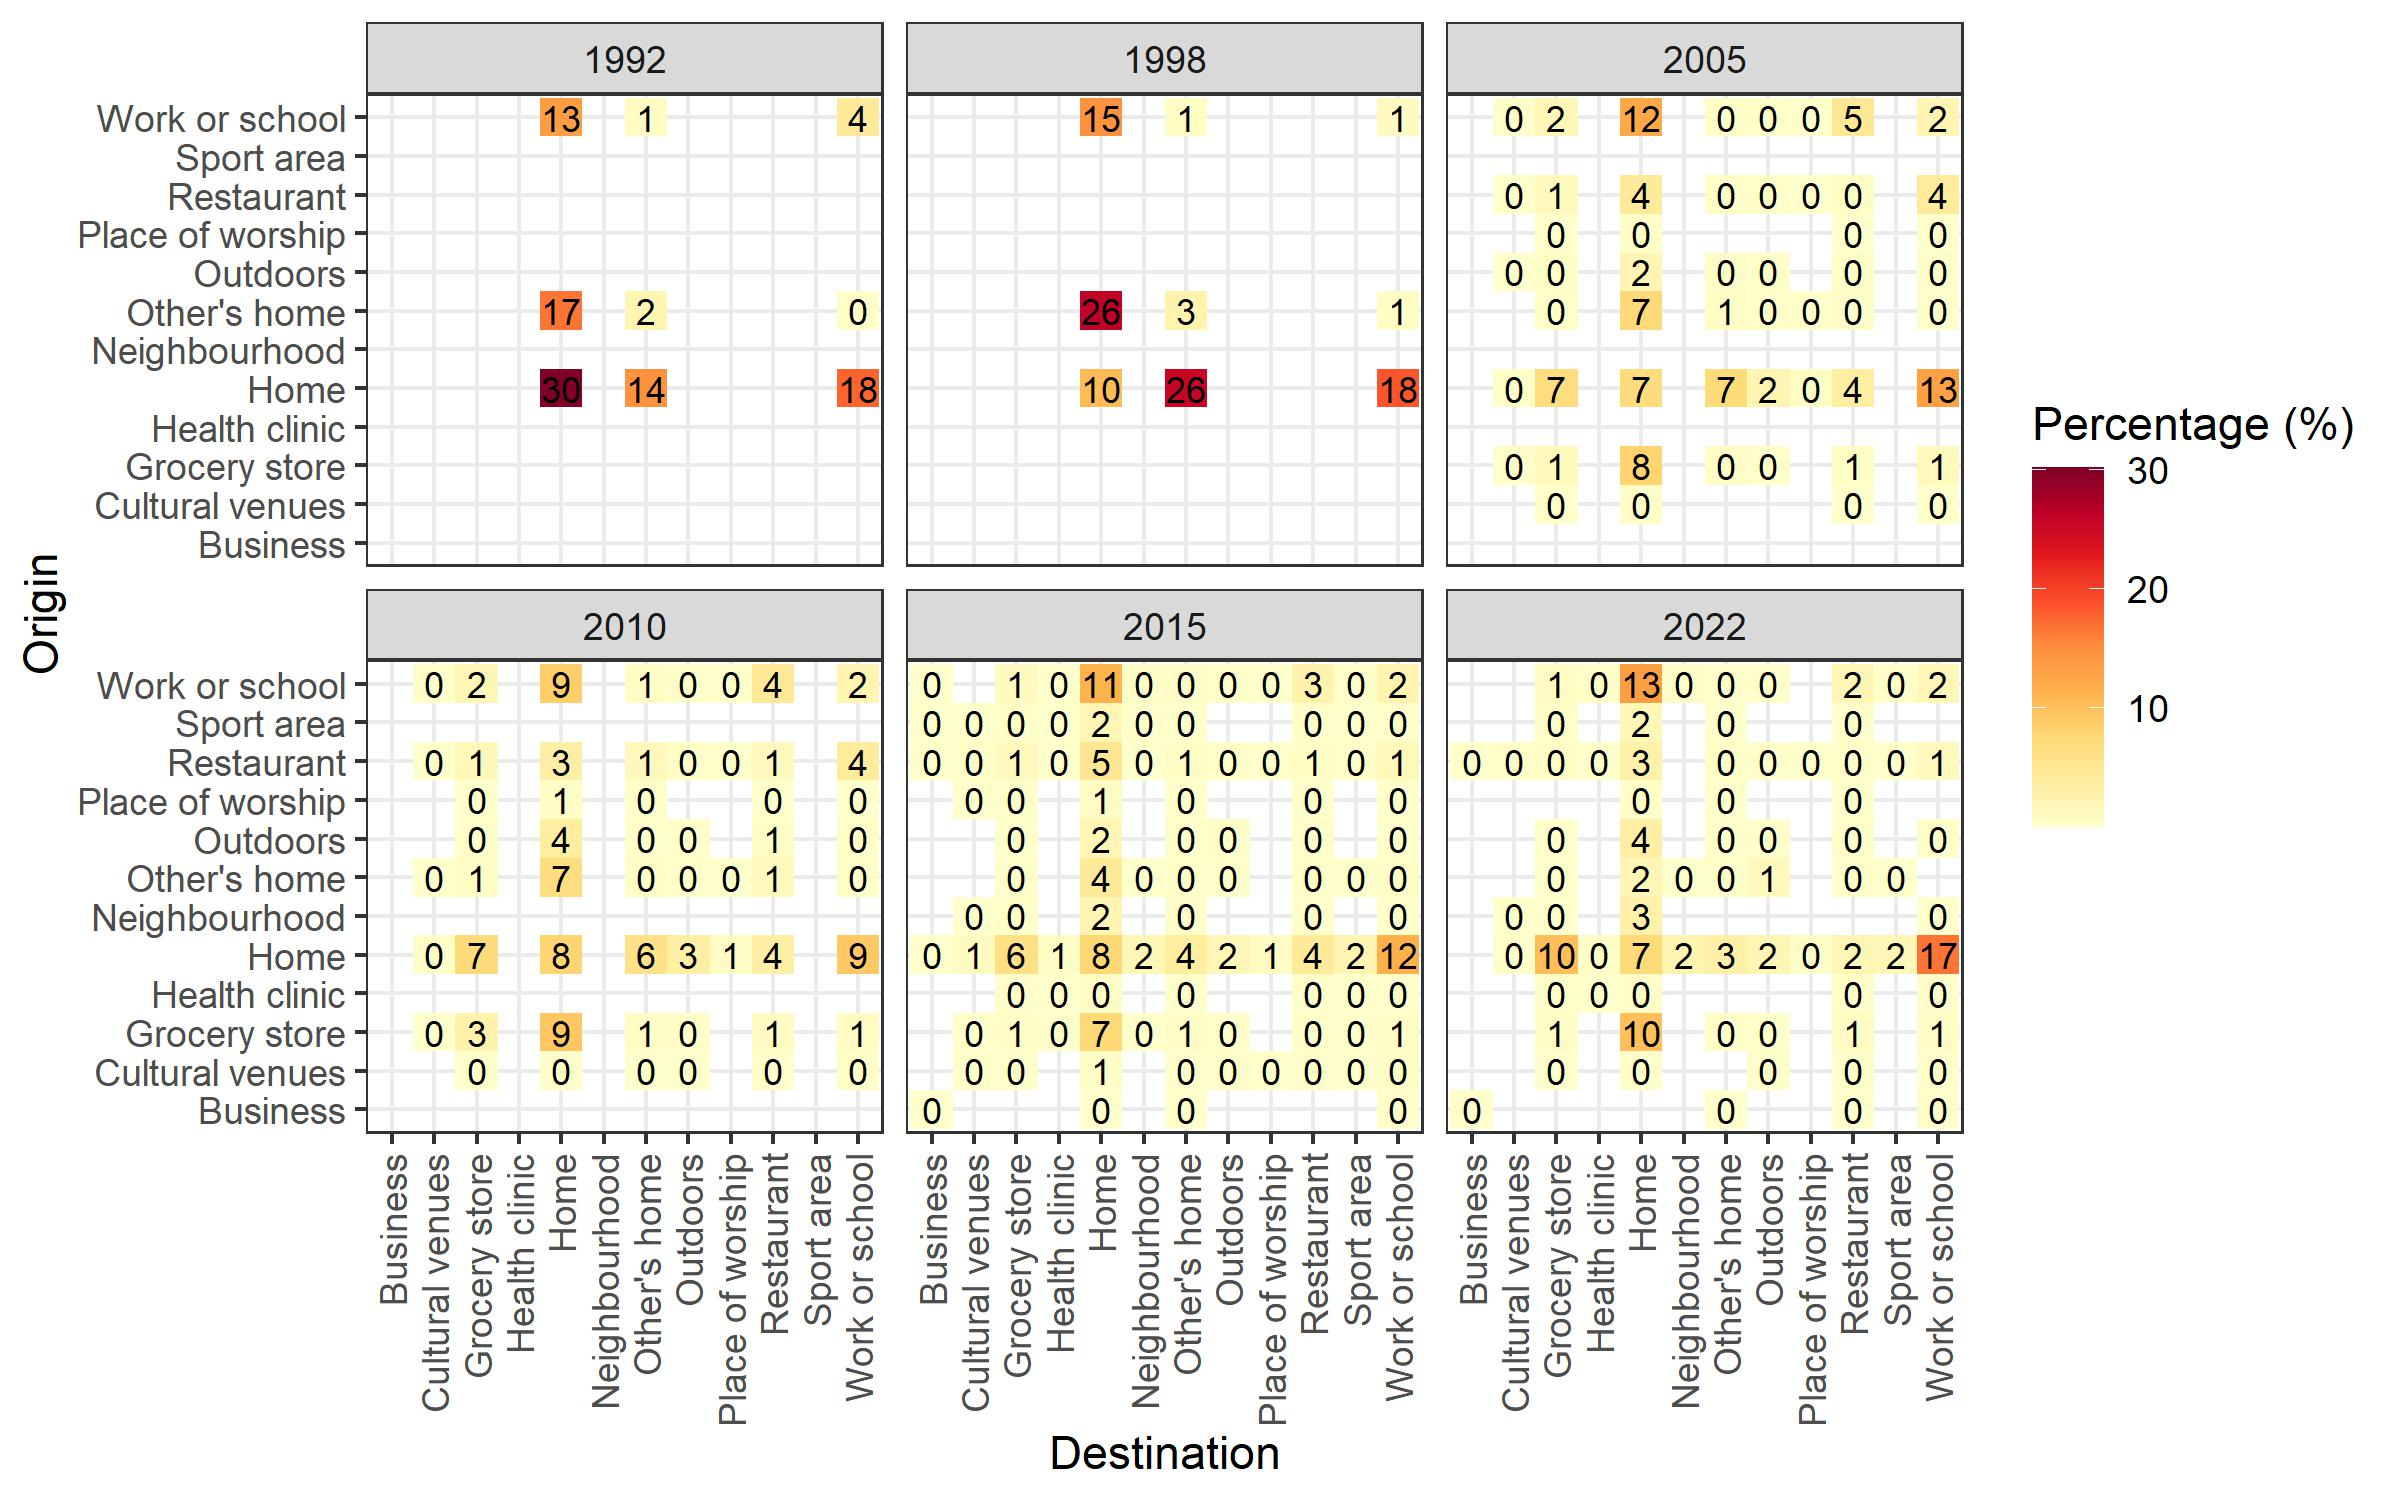
\includegraphics[width=1\linewidth]{figures/walking_hm_fig} \caption{Percentage of walking trips categorized by origin and destination}\label{fig:walking-heatmap}
\end{figure}

\begin{figure}
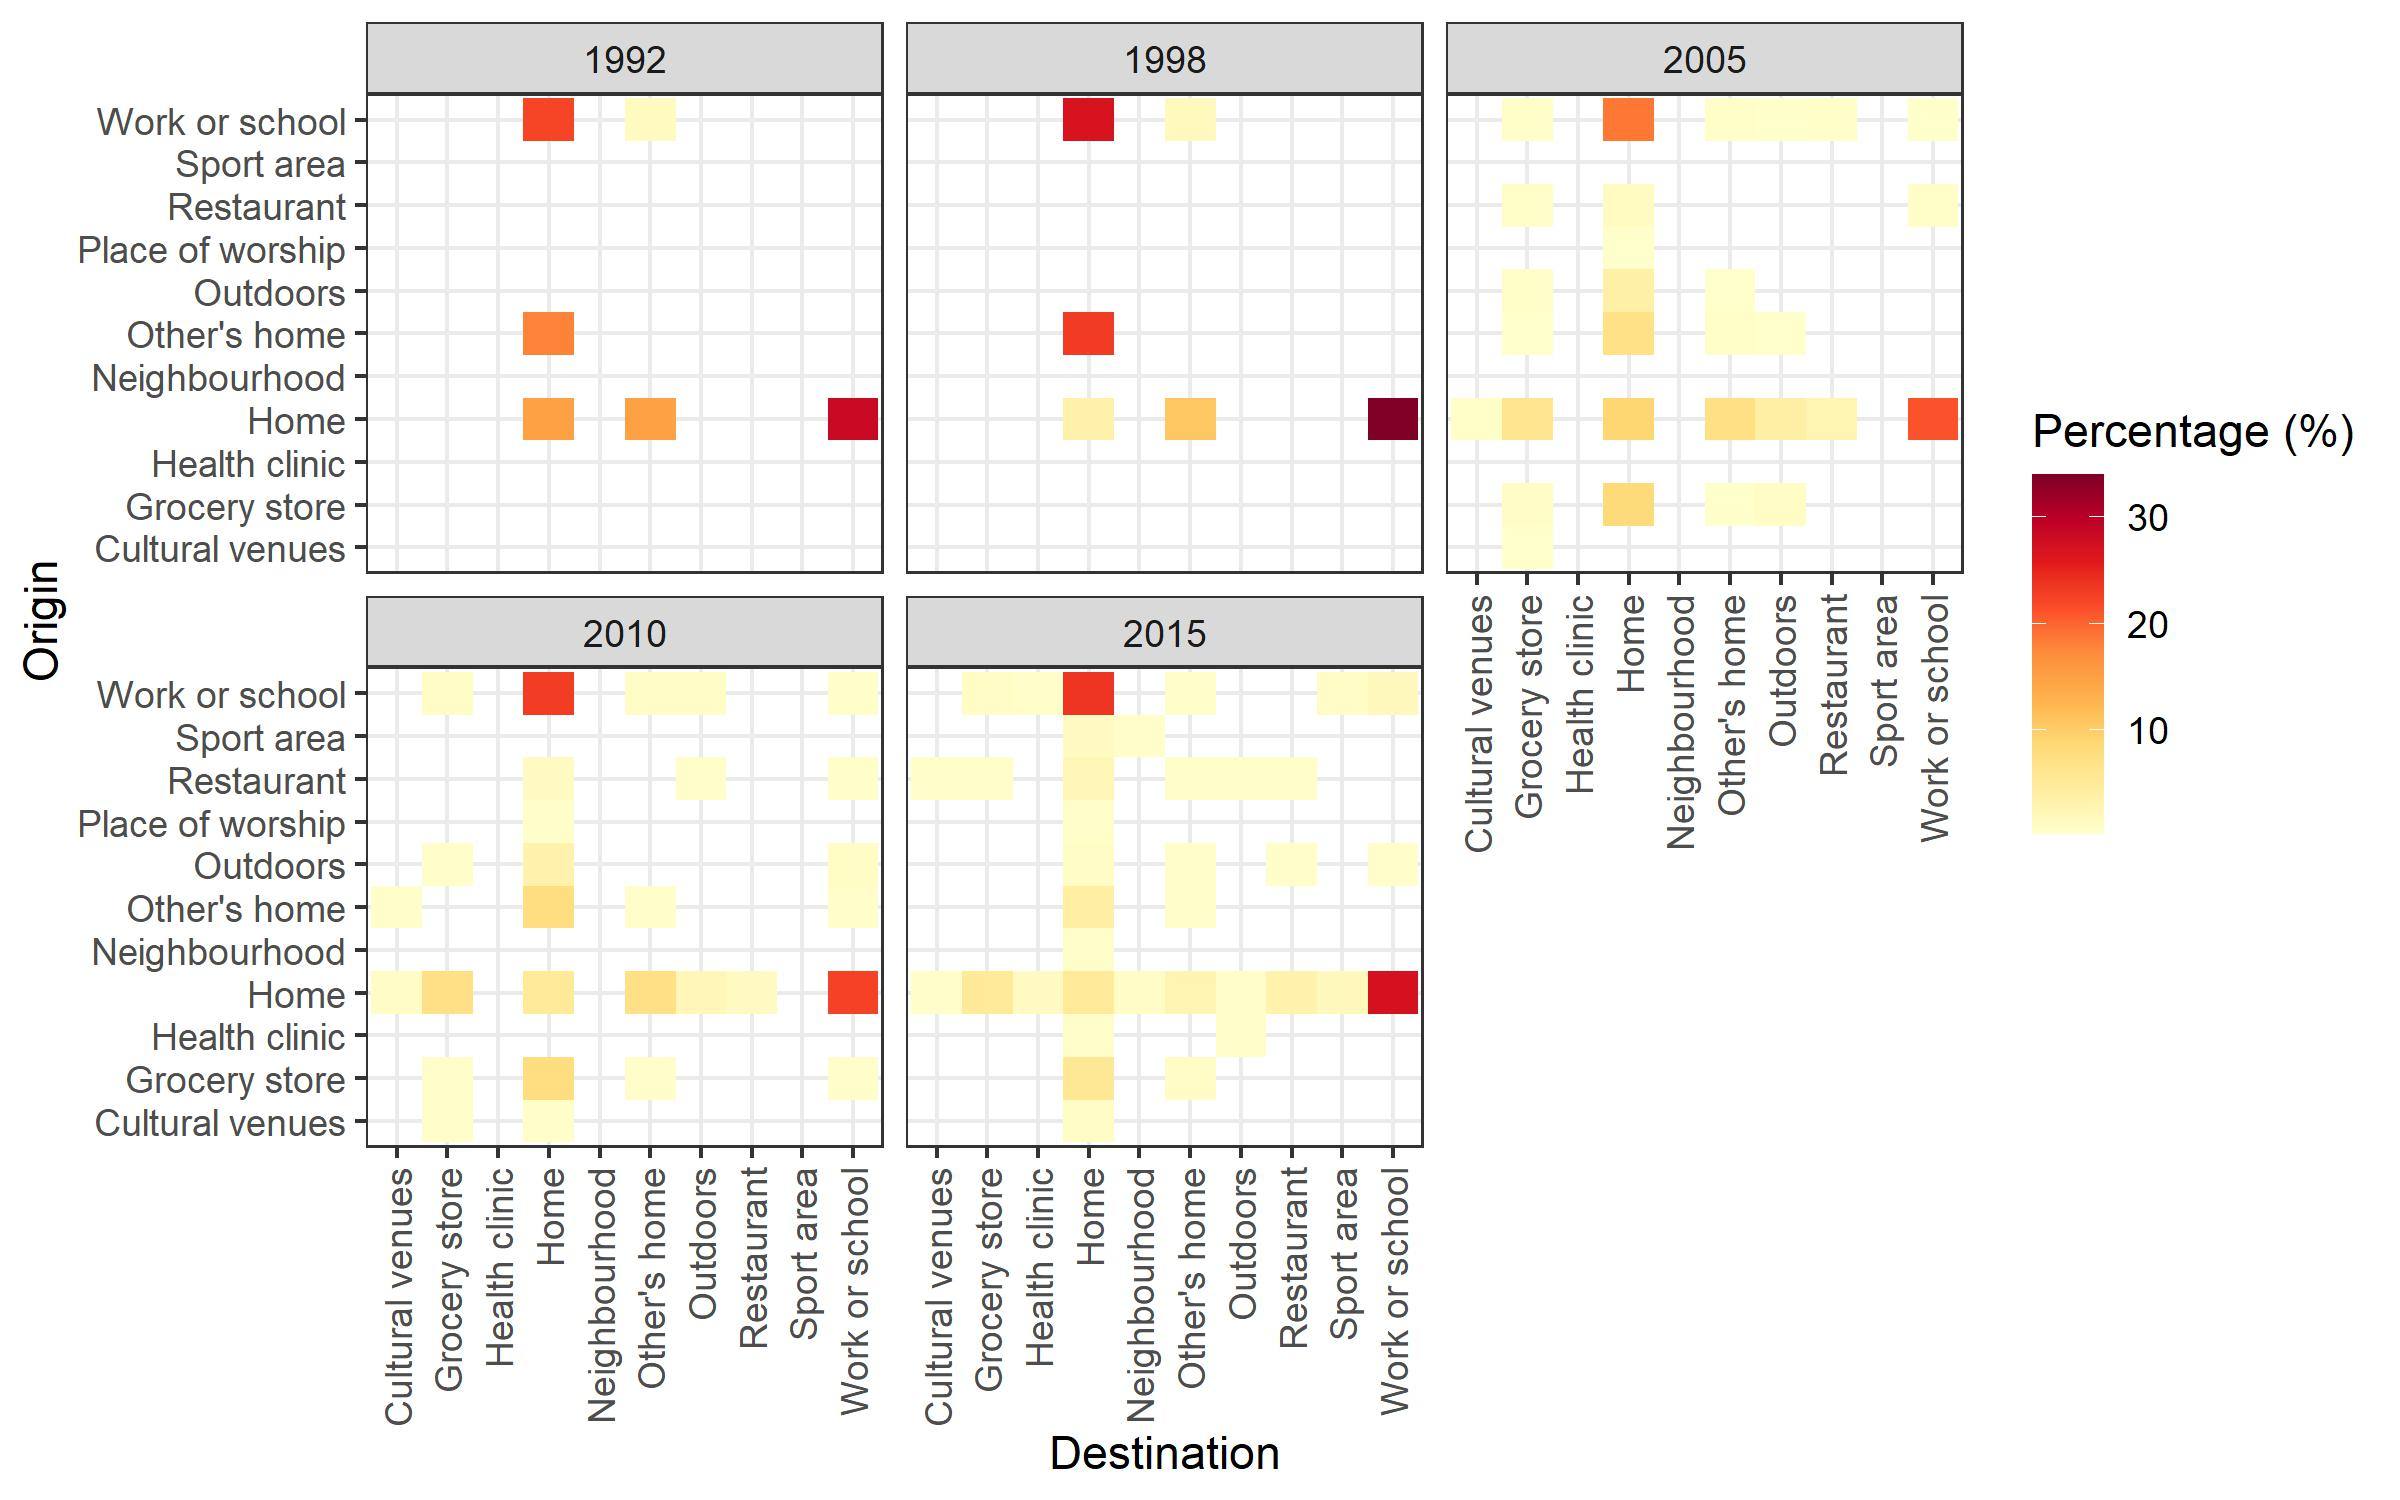
\includegraphics[width=1\linewidth]{figures/cycling_hm_fig} \caption{Percentage of walking trips categorized by origin and destination}\label{fig:cycling-heatmap}
\end{figure}

For cycling trips (Figure \ref{fig:cycling-heatmap}), in 1992, the most
common trip was from `Home' to `Work or school' (26\%), followed by
trips from `Other's home' to `Home' (22\%). In all following years, the
most frequent trip were between `Home' and `Work or school' in both
direction. This combination accounted for 65\% of the trips in 1998,
40\% in 2005, 52\% in 2010, and 58\% in 2015. However, in 2022, this
combination dropped to 43\%, mainly due to an increase in trips between
the ``Grocery store'' and ``Home'' (18\%). Additionally and unlike
walking trips, `Home' to `Home' trips were not a common cycling trip in
any of the surveys. This suggests that leisure trips, such as activities
around the home, are predominantly done by foot rather than by bicycle.

We analyzed whether the temporal differences in travel times for the
destinations were statistically significant. Only destinations that
appear in more than one survey year can have their temporal evolution
analyzed. Therefore, out of the twelve possible destinations, some
cycling locations could not be temporally analyzed: ``Business,''
``Neighborhood,'' and ``Place of worship.'' In the case of walking
trips, all destinations could be analyzed over time.

After performing the Kruskal-Wallis test (to assess whether there was a
statistically significant difference between the distributions of
empirical travel time values, considering the time differences for each
destination and the weight of each episode) and the pairwise Wilcoxon
test, we were able to identify the destinations where a statistically
significant difference was detected. Table \ref{tab:result-stats} shows
only the destinations where a statistically significant difference was
found, considering the two modes of active transport analyzed.

For both active transportation modes, the possible destinations had at
least two year with statistically significant difference in travel
times. Considering the cycling mode and, for instance, the ``Home''
destination, there was a statistically significant difference (p-value
\textless{} 2.2e-16) for every possible combination of two survey
cycles. This result indicates that the previously discussed increase in
typical cycling travel time for home destinations when compared 2022 to
2010 is statistically significant. As identified for cycling trips, all
destinations presented at least two years with statistically significant
difference in travel times for walking trips (p-value \textless{}
2.2e-16).

\begin{table}
\centering
\caption{\label{tab:kruskal-walking}\label{tab:result-stats}P-values of the pairwise Wilcoxon test.}
\centering
\resizebox{\ifdim\width>\linewidth\linewidth\else\width\fi}{!}{
\fontsize{10}{12}\selectfont
\begin{tabular}[t]{llllllll}
\toprule
Mode & Destination & Year & 1992 & 1998 & 2005 & 2010 & 2015\\
\midrule
 & Home & 1998 & 0.00e+00 & NA & NA & NA & NA\\

 & Home & 2005 & 0.00e+00 & 0.00e+00 & NA & NA & NA\\

 & Home & 2010 & 0.00e+00 & 0.00e+00 & 0.00e+00 & NA & NA\\

 & Home & 2015 & 0.00e+00 & 0.00e+00 & 0.00e+00 & 0.00e+00 & NA\\

 & Home & 2022 & 0.00e+00 & 0.00e+00 & 0.00e+00 & 0.00e+00 & 0.00e+00\\

 & Work or school & 1998 & 7.09e-211 & NA & NA & NA & NA\\

 & Work or school & 2005 & 0.00e+00 & 0.00e+00 & NA & NA & NA\\

 & Work or school & 2010 & 0.00e+00 & 0.00e+00 & 0.00e+00 & NA & NA\\

 & Work or school & 2015 & 0.00e+00 & 0.00e+00 & 0.00e+00 & 0.00e+00 & NA\\

 & Work or school & 2022 & 0.00e+00 & 0.00e+00 & 0.00e+00 & 0.00e+00 & 0.00e+00\\

 & Grocery store & 2010 & NA & NA & 0.00e+00 & NA & NA\\

 & Grocery store & 2015 & NA & NA & 0.00e+00 & 0.00e+00 & NA\\

 & Grocery store & 2022 & NA & NA & 0.00e+00 & 0.00e+00 & 0.00e+00\\

 & Neighbourhood & 2022 & NA & NA & NA & NA & 0.00e+00\\

 & Sport area & 2022 & NA & NA & NA & NA & 0.00e+00\\

 & Outdoors & 2010 & NA & NA & 4.33e-29 & NA & NA\\

 & Outdoors & 2015 & NA & NA & 0.00e+00 & 0.00e+00 & NA\\

 & Outdoors & 2022 & NA & NA & 0.00e+00 & 0.00e+00 & 0.00e+00\\

 & Restaurant & 2010 & NA & NA & 2.09e-295 & NA & NA\\

 & Restaurant & 2015 & NA & NA & 0.00e+00 & 0.00e+00 & NA\\

 & Restaurant & 2022 & NA & NA & 0.00e+00 & 0.00e+00 & 1.11e-179\\

 & Other's home & 1998 & 0.00e+00 & NA & NA & NA & NA\\

 & Other's home & 2005 & 0.00e+00 & 1.79e-83 & NA & NA & NA\\

 & Other's home & 2010 & 0.00e+00 & 0.00e+00 & 0.00e+00 & NA & NA\\

 & Other's home & 2015 & 0.00e+00 & 0.00e+00 & 0.00e+00 & 0.00e+00 & NA\\

 & Other's home & 2022 & 0.00e+00 & 0.00e+00 & 0.00e+00 & 0.00e+00 & 0.00e+00\\

 & Health clinic & 2022 & NA & NA & NA & NA & 4.12e-216\\

 & Cultural venues & 2010 & NA & NA & 4.52e-273 & NA & NA\\

 & Cultural venues & 2015 & NA & NA & 0.00e+00 & 0.00e+00 & NA\\

 & Cultural venues & 2022 & NA & NA & 0.00e+00 & 0.00e+00 & 0.00e+00\\

 & Place of worship & 2010 & NA & NA & 0.00e+00 & NA & NA\\

 & Place of worship & 2015 & NA & NA & 0.00e+00 & 0.00e+00 & NA\\

 & Place of worship & 2022 & NA & NA & 0.00e+00 & 0.00e+00 & 3.76e-18\\

\multirow[t]{-34}{*}{\raggedright\arraybackslash Walking} & Business & 2022 & NA & NA & NA & NA & 1.18e-305\\
\cmidrule{1-8}
 & Grocery store & 2010 & NA & NA & 0.00e+00 & NA & NA\\

 & Grocery store & 2015 & NA & NA & 0.00e+00 & 0.00e+00 & NA\\

 & Grocery store & 2022 & NA & NA & 0.00e+00 & 0.00e+00 & 0.00e+00\\

 & Home & 1998 & 1.08e-230 & NA & NA & NA & NA\\

 & Home & 2005 & 1.45e-24 & 0.00e+00 & NA & NA & NA\\

 & Home & 2010 & 0.00e+00 & 0.00e+00 & 0.00e+00 & NA & NA\\

 & Home & 2015 & 0.00e+00 & 8.44e-236 & 0.00e+00 & 0.00e+00 & NA\\

 & Home & 2022 & 0.00e+00 & 0.00e+00 & 0.00e+00 & 0.00e+00 & 0.00e+00\\

 & Work or school & 1998 & 0.00e+00 & NA & NA & NA & NA\\

 & Work or school & 2005 & 9.62e-228 & 0.00e+00 & NA & NA & NA\\

 & Work or school & 2010 & 1.30e-221 & 0.00e+00 & 0.00e+00 & NA & NA\\

 & Work or school & 2015 & 0.00e+00 & 0.00e+00 & 0.00e+00 & 0.00e+00 & NA\\

 & Work or school & 2022 & 0.00e+00 & 0.00e+00 & 0.00e+00 & 0.00e+00 & 0.00e+00\\

 & Health clinic & 2022 & NA & NA & NA & NA & 0.00e+00\\

 & Restaurant & 2010 & NA & NA & 1.03e-106 & NA & NA\\

 & Restaurant & 2015 & NA & NA & 0.00e+00 & 0.00e+00 & NA\\

 & Restaurant & 2022 & NA & NA & 0.00e+00 & 0.00e+00 & 0.00e+00\\

 & Sport area & 2022 & NA & NA & NA & NA & 0.00e+00\\

 & Outdoors & 2010 & NA & NA & 0.00e+00 & NA & NA\\

 & Outdoors & 2015 & NA & NA & 0.00e+00 & 0.00e+00 & NA\\

 & Outdoors & 2022 & NA & NA & 0.00e+00 & 0.00e+00 & 0.00e+00\\

 & Other's home & 1998 & 2.60e-122 & NA & NA & NA & NA\\

 & Other's home & 2005 & 0.00e+00 & 0.00e+00 & NA & NA & NA\\

 & Other's home & 2010 & 6.63e-41 & 0.00e+00 & 3.60e-287 & NA & NA\\

 & Other's home & 2015 & 4.03e-81 & 0.00e+00 & 5.62e-266 & 1.84e-148 & NA\\

 & Cultural venues & 2010 & NA & NA & 2.98e-142 & NA & NA\\

\multirow[t]{-27}{*}{\raggedright\arraybackslash Cycling} & Cultural venues & 2015 & NA & NA & 0.00e+00 & NA & NA\\
\bottomrule
\end{tabular}}
\end{table}

\subsubsection{Population with records of active
trip}\label{population-with-records-of-active-trip}

In general, the share of the population with active trip records varied
between 7.8\% and 14.6\% from 1992 to 2022 (Table
\ref{tab:pop-stats-table}). The year 1998 recorded the lowest level of
active trip participation, with 7.8\% (1,892,299 people), while 2010
marked the peak of active participation at 14.5\% (4,084,114 people). In
2015, the trend of increasing participation in walking and cycling trips
was reversed to the beginning of a decline, confirmed by the 2022
survey. In 2015, around 11\% of the population (3,265,846 people)
recorded at least one active trip. In 2022, this share of the population
fell to 8.9\%, the second lowest share in the entire historical series,
representing 2,856,564 people out of a total population of 32,136,802
people.

\begingroup\fontsize{6}{8}\selectfont

\begin{longtable}[t]{>{}lcccc>{}c|cccccc>{}c|cccccc}
\caption{\label{tab:pop-table-with-prevalence}\label{tab:pop-stats-table}Prevalence of active trip by transportation mode, year of analysis, gender and age group.}\\
\toprule
\multicolumn{1}{c}{ } & \multicolumn{6}{c}{Walking} & \multicolumn{6}{c}{Cycling} & \multicolumn{6}{c}{Walking and Cycling} \\
\cmidrule(l{3pt}r{3pt}){2-7} \cmidrule(l{3pt}r{3pt}){8-13} \cmidrule(l{3pt}r{3pt}){14-19}
  & 1992 & 1998 & 2005 & 2010 & 2015 & 2022 & 1992 & 1998 & 2005 & 2010 & 2015 & 2022 & 1992 & 1998 & 2005 & 2010 & 2015 & 2022\\
\midrule
\textbf{Total} & 8.112817 & 6.291682 & 13.184502 & 14.19945 & 10.908547 & 8.658299 & 1.0495040 & 0.6767230 & 0.9916221 & 1.1672734 & 0.9931890 & 0.8948529 & 9.105543 & 6.927465 & 14.059466 & 15.06081 & 11.648713 & 9.445029\\
\textbf{Men+} & 7.528134 & 5.034566 & 11.900550 & 13.92957 & 10.849674 & 8.888276 & 1.4451866 & 1.1804147 & 1.5584589 & 1.8666636 & 1.3415257 & 1.3262390 & 8.938127 & 6.182314 & 13.309461 & 15.30787 & 11.888698 & 10.054391\\
\textbf{Women+} & 8.693204 & 7.522666 & 14.421176 & 14.45877 & 10.965871 & 8.431012 & 0.6567284 & 0.1835012 & 0.4456571 & 0.4952302 & 0.6540139 & 0.4685109 & 9.271729 & 7.657127 & 14.781856 & 14.82340 & 11.415040 & 8.842793\\
\textbf{15 to 24 years} & 12.475414 & 8.382103 & 25.006727 & 22.27651 & 17.327913 & 19.884674 & 2.4992948 & 1.1562412 & 2.0781927 & 2.7505490 & 1.0582936 & 1.5829892 & 14.974709 & 9.295704 & 26.879289 & 24.01045 & 17.909552 & 21.467663\\
\textbf{25 to 34 years} & 7.152427 & 5.438087 & 13.328986 & 15.24494 & 14.802591 & 9.743730 & 1.6642883 & 0.4648541 & 1.1900530 & 1.1707246 & 1.5669562 & 1.6192238 & 8.816715 & 5.902941 & 14.280088 & 16.10988 & 15.778534 & 11.213176\\
\addlinespace
\textbf{35 to 44 years} & 5.786423 & 6.399745 & 10.517651 & 13.45598 & 9.381115 & 5.227927 & 0.6462726 & 1.1432400 & 1.0115445 & 1.0590734 & 1.1732797 & 0.8285441 & 6.243982 & 7.542986 & 11.428648 & 14.34433 & 10.495729 & 5.783006\\
\textbf{45 to 54 years} & 7.545398 & 5.901157 & 9.396331 & 11.68721 & 7.758093 & 5.705892 & 0.3033537 & 0.6276123 & 0.5064098 & 0.8438476 & 0.7483517 & 0.8156381 & 7.734909 & 6.528769 & 9.846246 & 12.35402 & 8.222011 & 6.302084\\
\textbf{55 to 64 years} & 8.893992 & 5.434284 & 9.611636 & 10.91250 & 7.696259 & 5.770591 & 0.2479165 & 0.2966514 & 0.9537762 & 0.8575569 & 0.7705951 & 0.4674650 & 9.141908 & 5.730936 & 10.484551 & 11.74650 & 8.432901 & 6.238056\\
\textbf{65 to 74 years} & 8.554111 & 5.269737 & 8.756855 & 11.59251 & 8.766450 & 6.658521 & 0.0000000 & 0.0000000 & 0.2241089 & 0.4235186 & 0.6987856 & 0.3335174 & 8.554111 & 5.269737 & 8.980964 & 11.81528 & 9.356414 & 6.960677\\
\textbf{75 years and over} & 5.915971 & 6.842840 & 13.543455 & 10.91263 & 8.626774 & 6.933773 & 0.0000000 & 0.0000000 & 0.0000000 & 0.0669363 & 0.5682477 & 0.0889275 & 5.915971 & 6.842840 & 13.543455 & 10.97957 & 9.195022 & 7.022700\\
\bottomrule
\end{longtable}
\endgroup{}

The decrease in the active population over the years is observed in both
genders, Men+ and Women+. However, the decline in the share of the
active population was more pronounced among Women+ than Men+, leading to
a shift in the pattern where Women+ had historically been the more
active gender. Women+ peaked at 14.82\% of the population with a record
of active episodes in 2010, but dropped to the second-lowest level of
8.84\% in 2022, only higher than 1998 when the active representation of
7.66\%. In contrast, Men+, who also peaked in 2010 with 15.31\% of the
population reporting active episodes, declined to 10.05\% in 2022,
appearing as the gender with higher active population share. When
analyzing by transportation mode, in all survey years a higher
proportion of Men+ reported at least one cycling episode on the previous
day compared to Women+ (ranging from 1.18\% to 1.87\% for Men+ and
0.18\% to 0.66\% for Women+). Conversely, Women+ historically reported
more walking trips than Men+, but this pattern changed in the most
recent survey (2022), reinforcing a trend already present in 2015. In
2022, 8.43\% of Women+ reported at least one walking episode, compared
to 8.89\% of Men+.

\begin{figure}
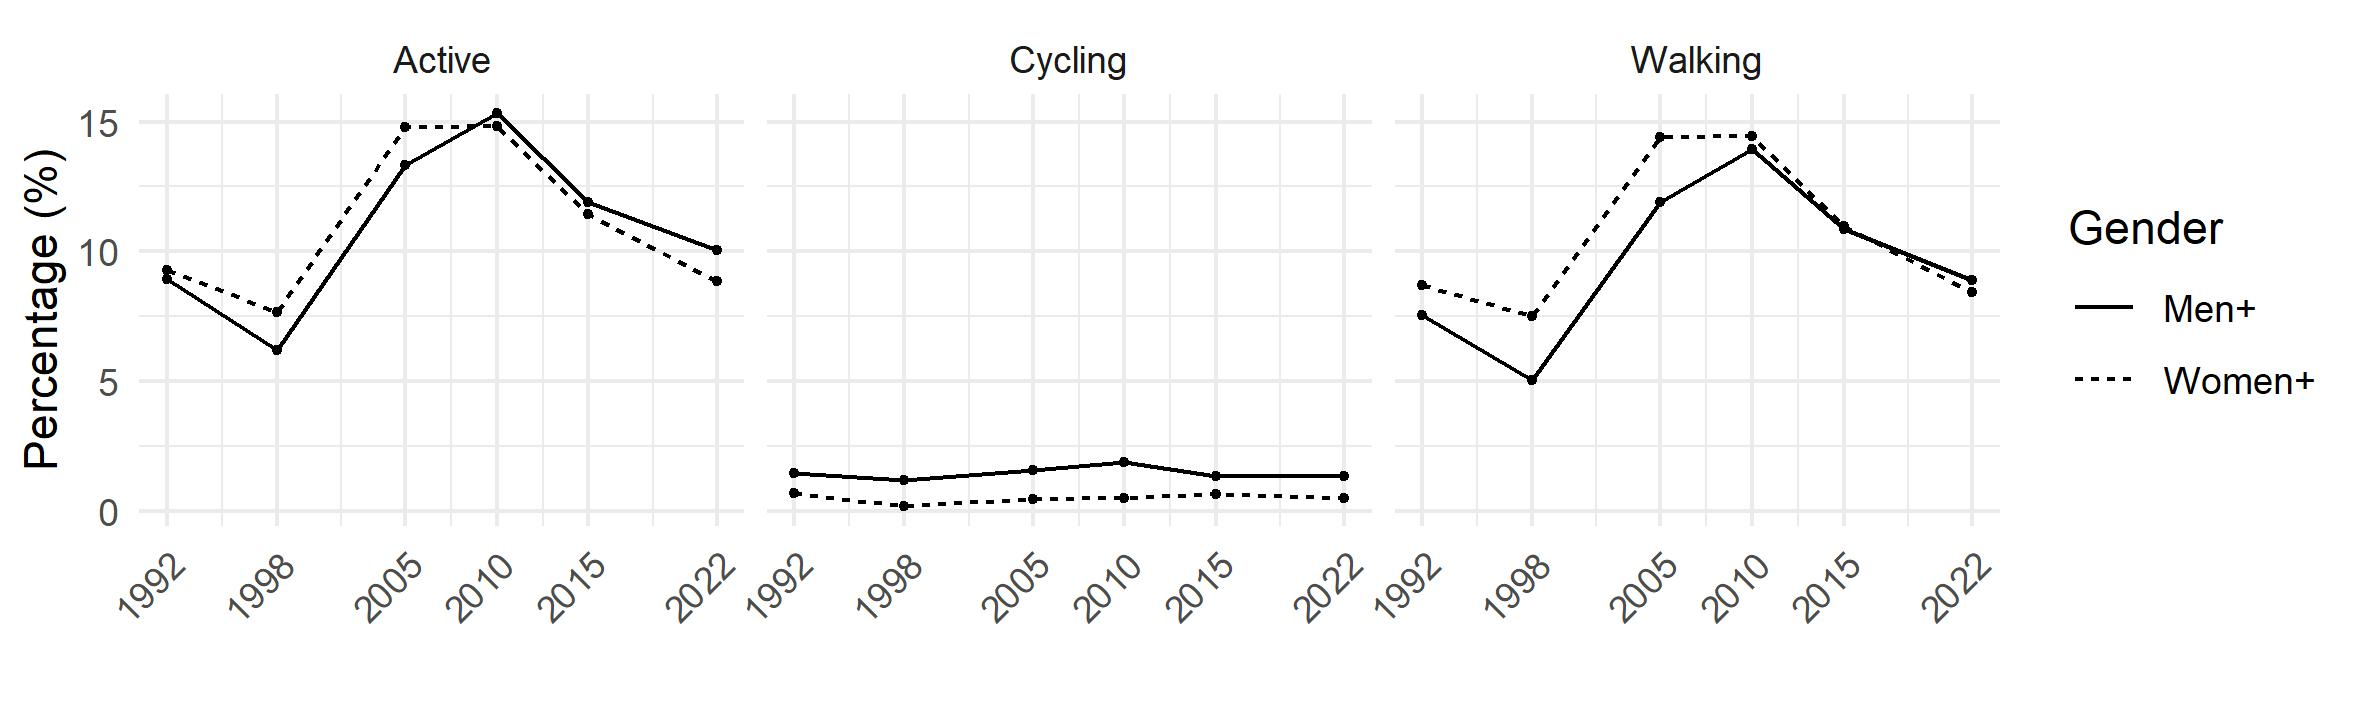
\includegraphics[width=1\linewidth]{figures/active_pop_gender_graph} \caption{Population with active trip episodes by transportation mode and gender.}\label{fig:gender-prevalence}
\end{figure}

When we analyze the population by age group, the youngest (those between
15 and 24 years) stand out as the most active group, ranging from 9.3\%
to 26.88\%, and marking 21.47\% in the most recent survey. This is the
only group that did not show a decrease in the prevalence of active
participation over the years, increasing from a low of 17.91\% in 2015
to 21.47\% in 2022 - although still below the levels recorded in 2010
(24.01\%) and 2005 (26.88\%). Historically, prevalence decreases as age
increases. However, in the most recent survey (2022), as well as in
2005, the oldest group (75 years and older) presented the third-highest
prevalence (7.02\%), surpassing the groups aged 35 to 44 years (5.78\%),
45 to 54 years (6.30\%), 55 to 64 years (6.24\%), and 65 to 74 years
(6.96\%).

The analysis by mode shows a similar trend. However, for cycling, the
second youngest group (aged 25 to 34 years) had the highest prevalence
in the 2022 survey (1.62\%), surpassing the youngest group (1.58\%). For
all other age groups, cycling prevalence decreases as age increases,
approaching 0\% for the oldest group (75 years and older).

\begin{figure}
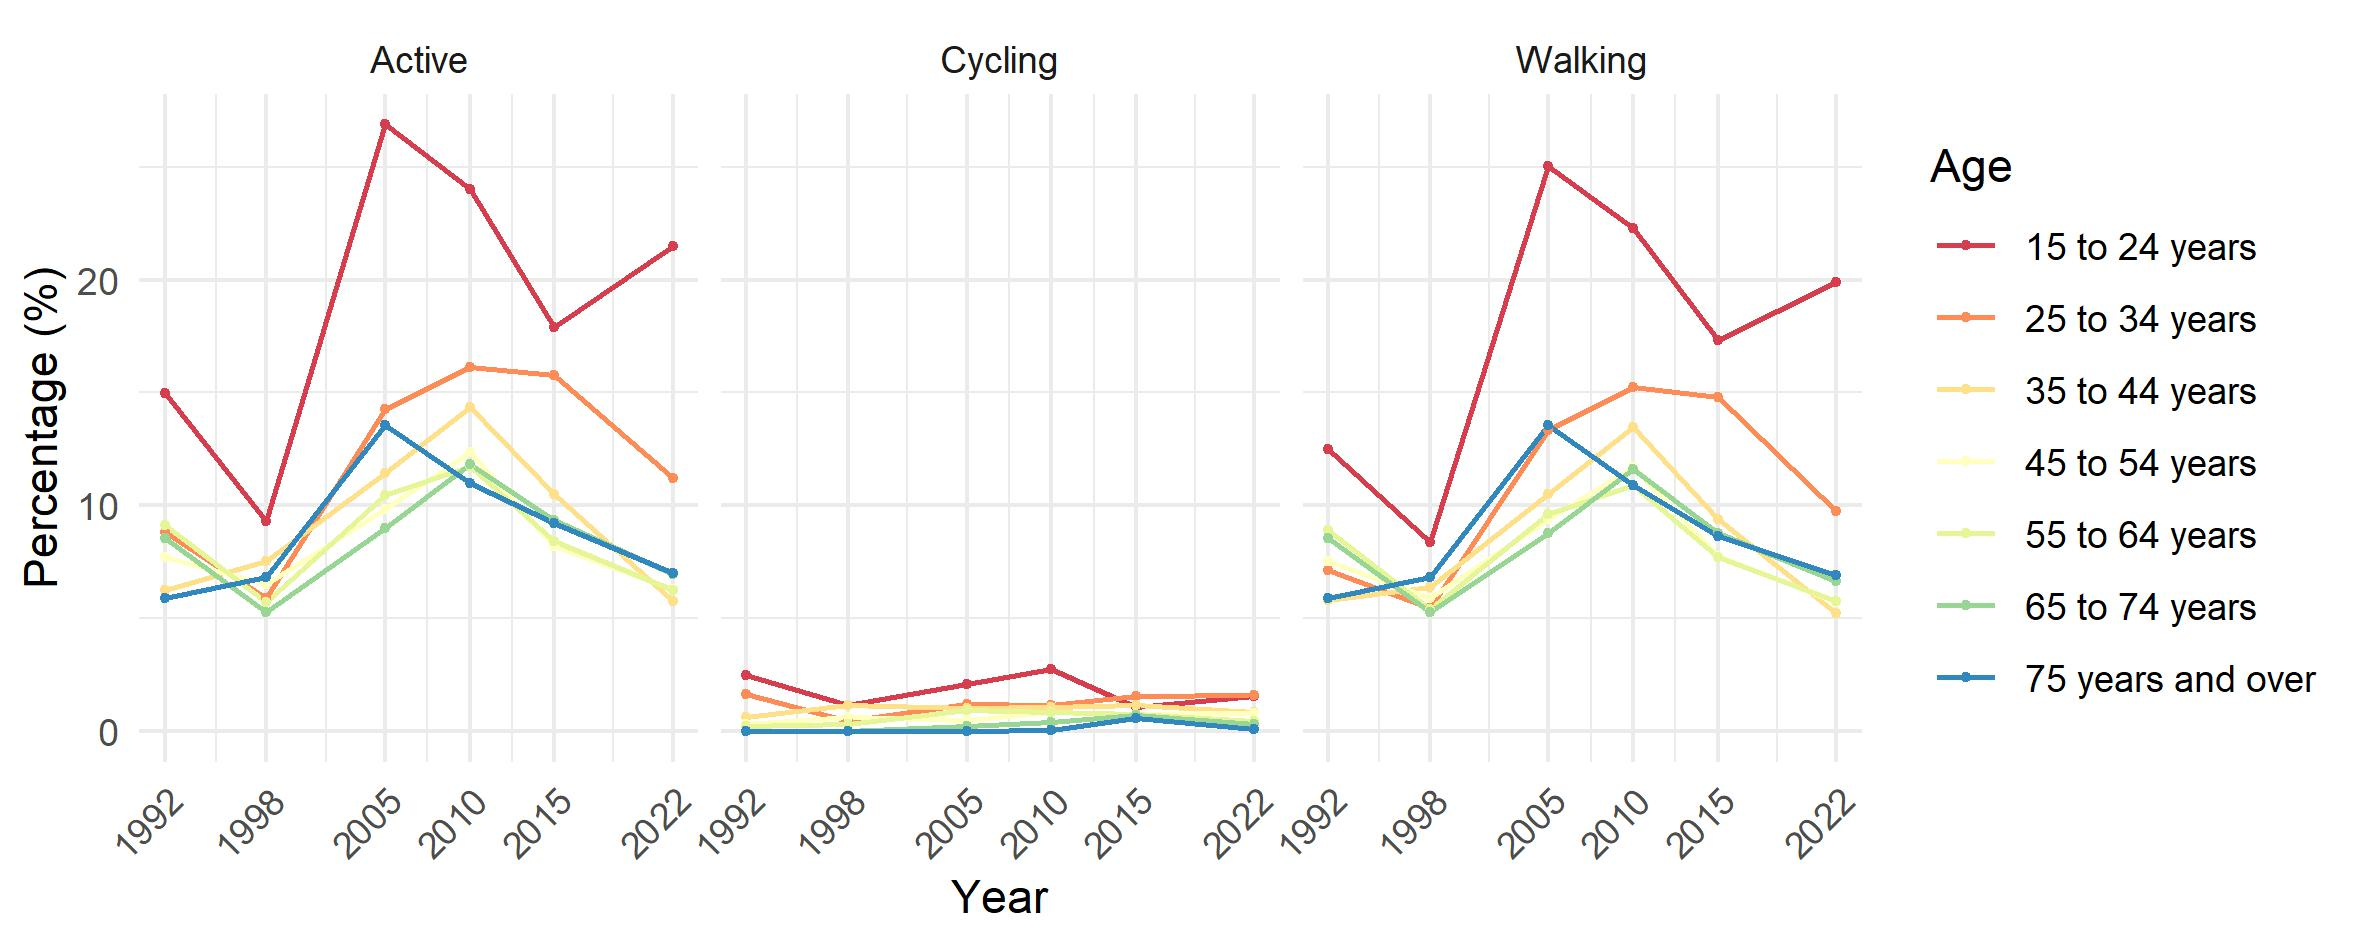
\includegraphics[width=1\linewidth]{figures/active_pop_age_graph} \caption{Population with active trip episodes by transportation mode and age group.}\label{fig:age-prevalence}
\end{figure}

The number of people with active trip episodes is mainly influenced by
walking episodes. On average, over 90\% of the recorded active trips
involve individuals with walking episodes. Analyzing the number of
episodes per person for the general population, the average value for
each year is approximately 0.22, ranging from a minimum of 0.15 in 1998
to a maximum of 0.30 in 2010. Considering only the population with
active episodes recorded, the average is around 2 active episodes per
person, varying from a maximum of 2.11 episodes in 2005 to a minimum of
1.77 episodes per person in 1992. The average of 2 episodes for the
active population is expected, as it reflects the two trips typically
required to travel to and from a specific location. Figure
\ref{fig:eps-per-person-fig} presents these values broken down by mode,
walking and cycling.

When we split the walking and cycling episodes by the active population
and the total population (Figure
\ref{fig:eps-per-person-act-total-fig}), we observe that each active
person recorded between 1.6 and 1.97 walking episodes, with the minimum
in 1992 and the maximum in 2005. This number dropped to 1.87 in 2015,
followed by a slight recovery to 1.91 in 2022. For cycling episodes,
considering only the active population, there has been an increasing
trend since 1998, rising from 0.14 to 0.20 cycling episodes per active
person in 2022. However, when we consider the total population, cycling
episodes remained stable at 0.02 episodes per person. Walking episodes
per total population showed the lowest value (0.17) since 1998, when the
minimum of 0.14 episodes per person was recorded.

\begin{figure}
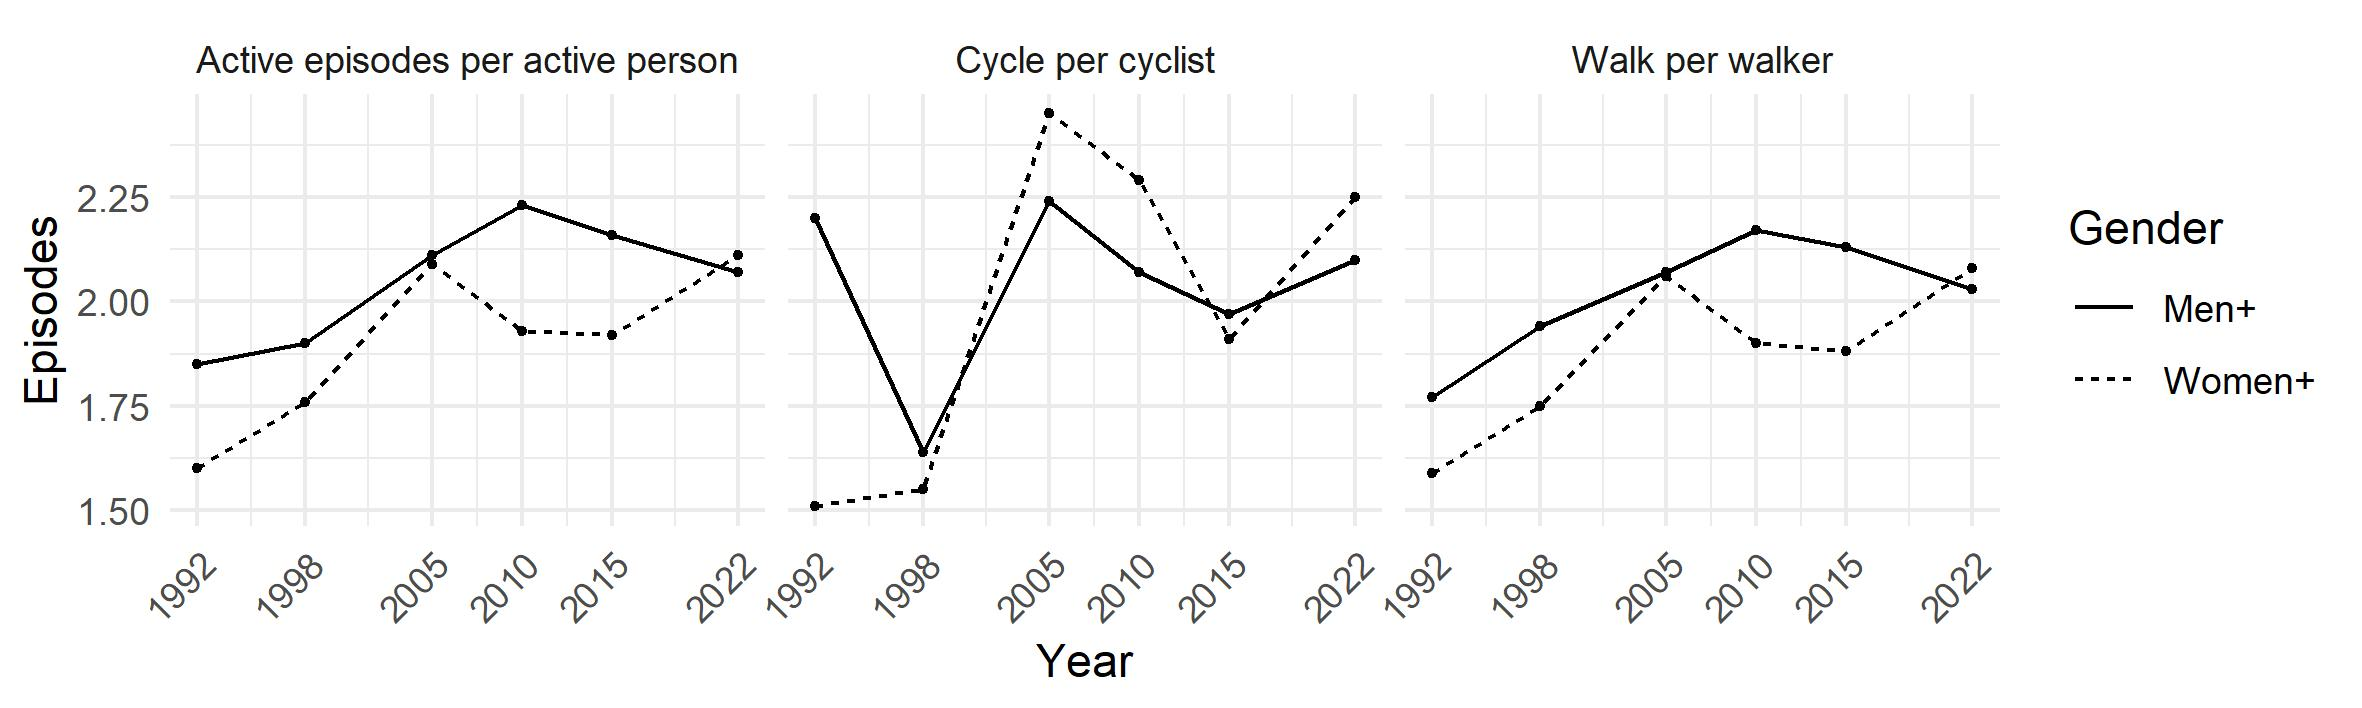
\includegraphics[width=1\linewidth]{figures/eps_gender_graph} \caption{Population with active trip episodes by transportation mode and gender.}\label{fig:gender-eps-prevalence}
\end{figure}

An interesting pattern emerges when we analyze the episodes by type of
active population (Figure \ref{fig:eps-per-person-by-mode-fig}). When we
divide the number of walking episodes by the population with recorded
walking trips (pedestrians), and the number of cycling episodes by the
population with recorded cycling trips (cyclists), we observe an
increasing trend for both rates. The results shown in Figures
\ref{fig:eps-per-person-act-total-fig} and
\ref{fig:eps-per-person-by-mode-fig}, along with the data on the
percentage of respondents with active trips, indicate that: first, the
number of people with active episodes has been decreasing over time;
however, among those with recorded active trips, the number of episodes
per person is increasing for both transportation modes, walking and
cycling.

\begin{figure}
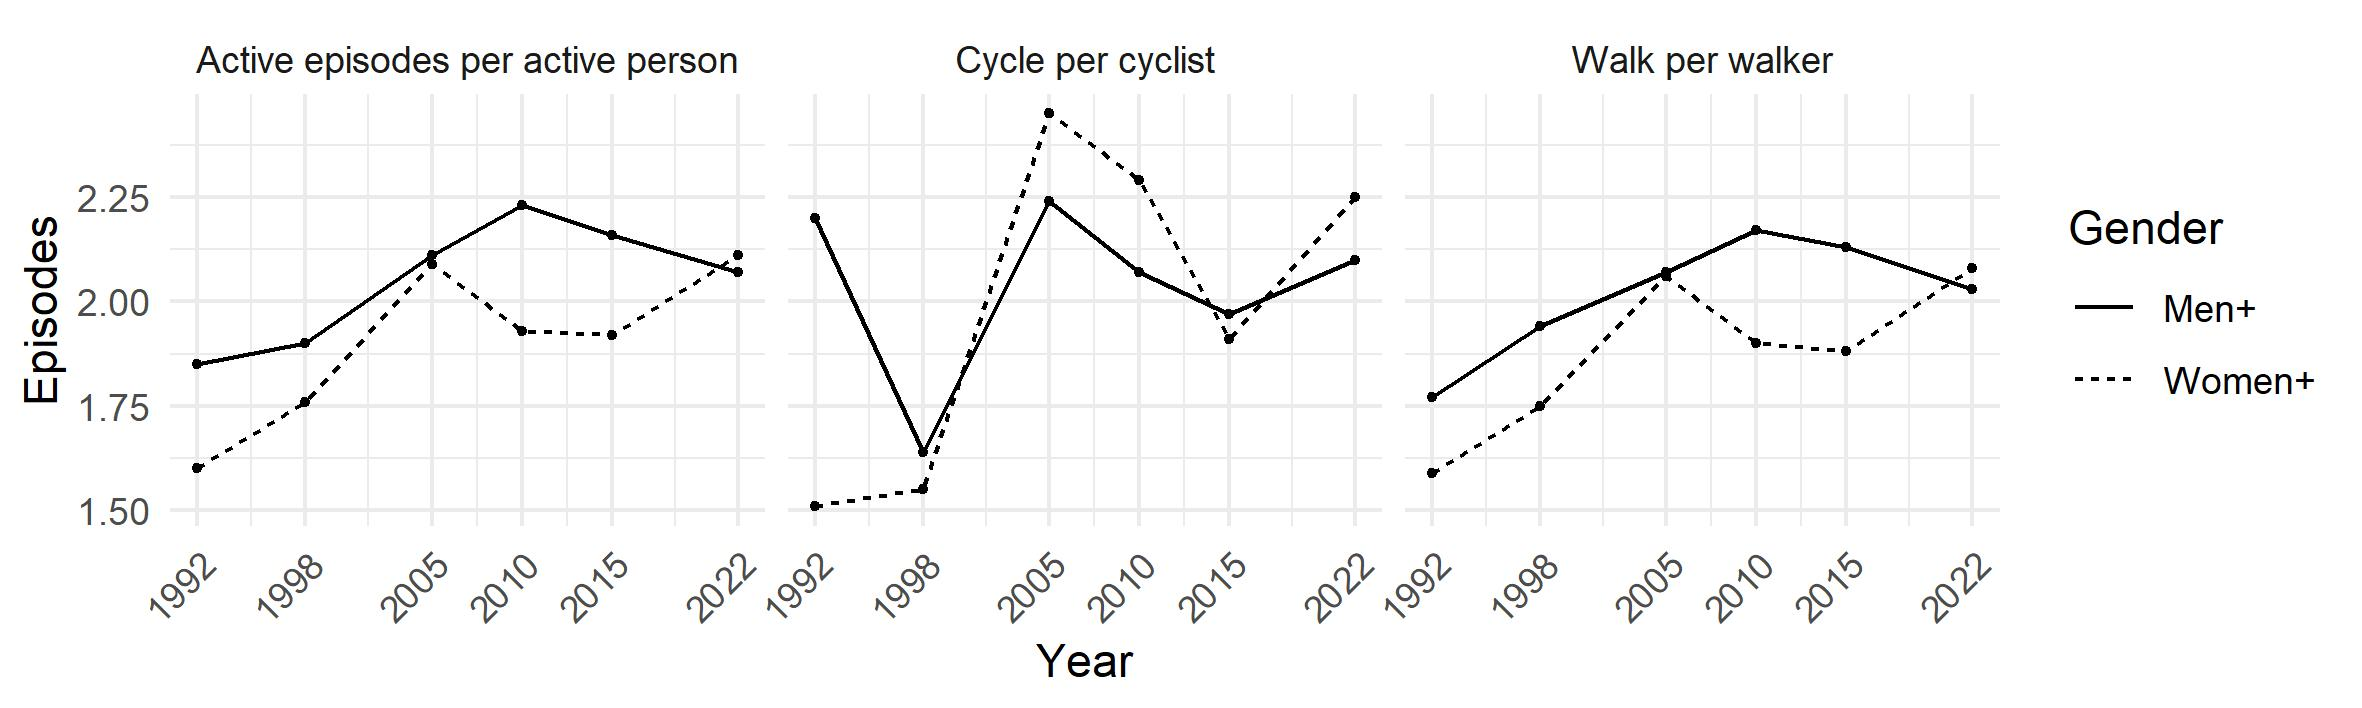
\includegraphics[width=1\linewidth]{figures/eps_gender_graph} \caption{Population with active trip episodes by transportation mode and age group.}\label{fig:age-eps-figure}
\end{figure}

\subsection{Calibrated impedance
function}\label{calibrated-impedance-function}

After analyzing the active travel episodes and population with records
of active trip, this section presents the identified impedance functions
for walking and cycling trips to various destinations across CMA/CA in
Canada from 1992 to 2022. In general, the impedance functions aim to
capture transportation behavior, illustrating that the likelihood of
traveling between two points decreases as travel duration increases.
Each impedance function follows one of the mathematical equations
previously mentioned, enabling the plotting of PDF curves. These curves
also highlight critical points at which a person's tendency to walk or
cycle significantly decreases.

As explained in the methodology section, we used the
\texttt{fitdistrplus} package \citep{delignette2015fitdistrplus} to
calibrate the functions. We selected the best impedance function for
each transportation mode, destination, and year based on the lowest
Akaike Information Criterion (AIC) value \citep{akaike1974}. The AIC
metric not only assesses the goodness of fit but also penalizes model
complexity to prevent overfitting. AIC provides a balance between a
model's accuracy and simplicity, with lower values indicating a more
economical model. The distribution with the lowest AIC was considered
the most suitable for representing the distance decay curve for each
specific destination in each year. We chose AIC as the selection
criterion because, while the \texttt{fitdistrplus} package accommodates
weighted episodes during estimation, it does not extend this
functionality to diagnostic plots, which are typically unweighted and
traditionally used to select the best-fitting function.

In total, we fitted 83 impedance functions. Among the candidate
distributions, only the negative exponential type was not selected. The
absence of exponential functions, given the variety of destinations,
year and mode of transport, indicates that the impedance functions
applied in active accessibility studies may not be adequately measuring
travel behavior, especially for cases when the travel time is close to 0
minute. Table \ref{tab:walking-functions-tab} displays the selected
functions for walking trips, while Table \ref{tab:cycling-functions-tab}
presents the functions for cycling trips. Appendix A includes the AIC,
BIC, and log-likelihood values for all candidate distributions.

\begin{table}
\centering
\caption{\label{tab:selected_functions}\label{tab:walking-functions-tab}Impedance functions and AIC for walking trips.}
\centering
\resizebox{\ifdim\width>\linewidth\linewidth\else\width\fi}{!}{
\fontsize{10}{12}\selectfont
\begin{threeparttable}
\begin{tabular}[t]{rllrrrr}
\toprule
\multicolumn{1}{c}{\textbf{Year}} & \multicolumn{1}{c}{\textbf{Destination}} & \multicolumn{1}{c}{\textbf{Impedance function}} & \multicolumn{1}{c}{\textbf{Parameter 1*}} & \multicolumn{1}{c}{\textbf{Parameter 2*}} & \multicolumn{1}{c}{\textbf{AIC}} & \multicolumn{1}{c}{\textbf{Count}}\\
\midrule
 & Home & Lognormal & 2.92 & 0.77 & 7761103 & 296\\

 & Other's home & Lognormal & 2.15 & 0.84 & 1778150 & 81\\

\multirow[t]{-3}{*}{\raggedleft\arraybackslash 1992} & Work or school & Lognormal & 2.38 & 0.70 & 2319400 & 113\\
\cmidrule{1-7}
 & Home & Lognormal & 2.07 & 0.92 & 5656275 & 302\\

 & Other's home & Lognormal & 1.75 & 0.97 & 2892771 & 176\\

\multirow[t]{-3}{*}{\raggedleft\arraybackslash 1998} & Work or school & Gamma & 1.23 & 0.09 & 2318752 & 109\\
\cmidrule{1-7}
 & Cultural venues & Gamma & 4.10 & 0.34 & 238506 & 25\\

 & Grocery store & Gamma & 1.22 & 0.10 & 4776215 & 558\\

 & Home & Gamma & 1.16 & 0.08 & 17291041 & 1831\\

 & Other's home & Gamma & 1.03 & 0.11 & 3420742 & 436\\

 & Outdoors & Gamma & 1.24 & 0.13 & 1272012 & 155\\

 & Place of worship & Gamma & 2.07 & 0.19 & 228307 & 32\\

 & Restaurant & Lognormal & 1.95 & 0.79 & 3727576 & 421\\

\multirow[t]{-8}{*}{\raggedleft\arraybackslash 2005} & Work or school & Lognormal & 2.13 & 0.79 & 8182691 & 724\\
\cmidrule{1-7}
 & Cultural venues & Gamma & 3.60 & 0.34 & 304141 & 25\\

 & Grocery store & Lognormal & 2.08 & 0.85 & 6369652 & 489\\

 & Home & Gamma & 1.10 & 0.07 & 19584386 & 1424\\

 & Other's home & Lognormal & 1.81 & 0.92 & 4035574 & 336\\

 & Outdoors & Gamma & 1.27 & 0.13 & 2114346 & 167\\

 & Place of worship & Lognormal & 1.95 & 0.70 & 285177 & 28\\

 & Restaurant & Lognormal & 2.01 & 0.90 & 5187191 & 371\\

\multirow[t]{-8}{*}{\raggedleft\arraybackslash 2010} & Work or school & Lognormal & 2.21 & 0.78 & 7917431 & 494\\
\cmidrule{1-7}
 & Business & Lognormal & 2.41 & 0.67 & 102286 & 8\\

 & Cultural venues & Gamma & 4.57 & 0.34 & 543242 & 43\\

 & Grocery store & Lognormal & 2.48 & 0.68 & 4001111 & 338\\

 & Health clinic & Lognormal & 2.44 & 0.70 & 324578 & 27\\

 & Home & Lognormal & 2.57 & 0.74 & 17235960 & 1202\\

 & Neighbourhood & Lognormal & 2.41 & 0.77 & 981626 & 53\\

 & Other's home & Lognormal & 2.43 & 0.80 & 2388598 & 186\\

 & Outdoors & Lognormal & 2.54 & 0.79 & 1247963 & 72\\

 & Place of worship & Gamma & 5.64 & 0.28 & 343187 & 24\\

 & Restaurant & Lognormal & 2.38 & 0.74 & 3490082 & 231\\

 & Sport area & Lognormal & 2.48 & 0.59 & 1199687 & 94\\

\multirow[t]{-12}{*}{\raggedleft\arraybackslash 2015} & Work or school & Lognormal & 2.55 & 0.64 & 6612061 & 407\\
\cmidrule{1-7}
 & Business & Uniform & 0.00 & 20.97 & 56268 & 5\\

 & Cultural venues & Gamma & 3.89 & 0.24 & 157354 & 12\\

 & Grocery store & Lognormal & 2.78 & 0.62 & 4618945 & 192\\

 & Health clinic & Lognormal & 2.40 & 0.98 & 325649 & 12\\

 & Home & Lognormal & 2.80 & 0.67 & 16787347 & 633\\

 & Neighbourhood & Lognormal & 2.28 & 0.88 & 963957 & 33\\

 & Other's home & Lognormal & 2.23 & 0.80 & 1463414 & 86\\

 & Outdoors & Lognormal & 2.27 & 0.77 & 1313257 & 43\\

 & Place of worship & Uniform & 0.00 & 33.68 & 160837 & 11\\

 & Restaurant & Lognormal & 2.37 & 0.70 & 2098269 & 100\\

 & Sport area & Lognormal & 2.63 & 0.45 & 651353 & 39\\

\multirow[t]{-12}{*}{\raggedleft\arraybackslash 2022} & Work or school & Lognormal & 2.64 & 0.63 & 7432435 & 192\\
\bottomrule
\end{tabular}
\begin{tablenotes}
\item \textit{Note: } 
\item For 'lnorm' distributions, 'Parameter 1' and 'Parameter 2' refer to the mean and standard deviation of the distribution on the logarithmic scaler, respectively. For the 'Gamma' distribution, 'Parameter 1' and 'Parameter 2' refer to the rate and shape of the distribution, respectively. For the 'Uniform' distribution,  'Parameter 1' refers to the minimum lower bound and 'Parameter 2'  refers to the upper bound (maximum) of the distribution.  'AIC' means Akaike information criterion.
\end{tablenotes}
\end{threeparttable}}
\end{table}

\begin{table}
\centering
\caption{\label{tab:selected_functions}\label{tab:cycling-functions-tab}Impedance functions and AIC for cycling trips.}
\centering
\resizebox{\ifdim\width>\linewidth\linewidth\else\width\fi}{!}{
\fontsize{10}{12}\selectfont
\begin{threeparttable}
\begin{tabular}[t]{rllrrrr}
\toprule
\multicolumn{1}{c}{\textbf{Year}} & \multicolumn{1}{c}{\textbf{Destination}} & \multicolumn{1}{c}{\textbf{Impedance function}} & \multicolumn{1}{c}{\textbf{Parameter 1*}} & \multicolumn{1}{c}{\textbf{Parameter 2*}} & \multicolumn{1}{c}{\textbf{AIC}} & \multicolumn{1}{c}{\textbf{Count}}\\
\midrule
 & Home & Gamma & 1.18 & 0.05 & 1018747 & 37\\

 & Other's home & Lognormal & 2.57 & 0.82 & 373451 & 11\\

\multirow[t]{-3}{*}{\raggedleft\arraybackslash 1992} & Work or school & Gamma & 3.00 & 0.17 & 433582 & 19\\
\cmidrule{1-7}
 & Home & Gamma & 1.70 & 0.07 & 715802 & 30\\

 & Other's home & Lognormal & 2.79 & 0.80 & 113905 & 7\\

\multirow[t]{-3}{*}{\raggedleft\arraybackslash 1998} & Work or school & Gamma & 3.37 & 0.10 & 481536 & 19\\
\cmidrule{1-7}
 & Cultural venues & Uniform & 0.00 & 15.13 & 6355 & 2\\

 & Grocery store & Gamma & 1.93 & 0.14 & 320218 & 29\\

 & Home & Gamma & 1.49 & 0.07 & 1794317 & 140\\

 & Other's home & Gamma & 1.84 & 0.15 & 310058 & 27\\

 & Outdoors & Gamma & 2.99 & 0.17 & 215894 & 17\\

 & Restaurant & Gamma & 3.37 & 0.21 & 109072 & 10\\

\multirow[t]{-7}{*}{\raggedleft\arraybackslash 2005} & Work or school & Lognormal & 2.93 & 0.70 & 888655 & 64\\
\cmidrule{1-7}
 & Cultural venues & Uniform & 0.00 & 32.58 & 38938 & 3\\

 & Grocery store & Lognormal & 2.68 & 0.61 & 315037 & 20\\

 & Home & Lognormal & 2.60 & 0.77 & 2006242 & 103\\

 & Other's home & Lognormal & 2.40 & 0.63 & 338777 & 19\\

 & Outdoors & Lognormal & 2.05 & 0.59 & 92699 & 8\\

 & Restaurant & Uniform & 0.00 & 17.49 & 35370 & 3\\

\multirow[t]{-7}{*}{\raggedleft\arraybackslash 2010} & Work or school & Lognormal & 2.65 & 0.77 & 1292760 & 53\\
\cmidrule{1-7}
 & Cultural venues & Lognormal & 2.71 & 0.00 & -Inf & 2\\

 & Grocery store & Lognormal & 3.08 & 0.80 & 229413 & 14\\

 & Health clinic & Lognormal & 2.93 & 0.86 & 80810 & 4\\

 & Home & Lognormal & 3.08 & 0.61 & 1745846 & 98\\

 & Neighbourhood & Uniform & 0.00 & 48.55 & 49924 & 3\\

 & Other's home & Lognormal & 2.52 & 0.44 & 140210 & 12\\

 & Outdoors & Uniform & 0.00 & 35.03 & 31463 & 3\\

 & Restaurant & Lognormal & 3.11 & 0.60 & 115406 & 9\\

 & Sport area & Uniform & 0.00 & 17.47 & 32969 & 6\\

\multirow[t]{-10}{*}{\raggedleft\arraybackslash 2015} & Work or school & Lognormal & 3.03 & 0.41 & 1162876 & 63\\
\cmidrule{1-7}
 & Grocery store & norm & 47.03 & 20.72 & 602645 & 8\\

 & Health clinic & Uniform & 0.00 & 61.98 & 123138 & 3\\

 & Home & Gamma & 4.04 & 0.15 & 1798770 & 56\\

 & Outdoors & Lognormal & 3.44 & 0.11 & 94804 & 2\\

 & Restaurant & norm & 26.29 & 5.83 & 100585 & 3\\

 & Sport area & norm & 29.89 & 17.05 & 124824 & 5\\

\multirow[t]{-7}{*}{\raggedleft\arraybackslash 2022} & Work or school & Gamma & 5.87 & 0.24 & 832953 & 37\\
\bottomrule
\end{tabular}
\begin{tablenotes}
\item \textit{Note: } 
\item For 'lnorm' distributions, 'Parameter 1' and 'Parameter 2' refer to the mean and standard deviation of the distribution on the logarithmic scaler, respectively. For the 'Gamma' distribution, 'Parameter 1' and 'Parameter 2' refer to the rate and shape of the distribution, respectively. For the 'Uniform' distribution,  'Parameter 1' refers to the minimum lower bound and 'Parameter 2'  refers to the upper bound (maximum) of the distribution.  'AIC' means Akaike information criterion.
\end{tablenotes}
\end{threeparttable}}
\end{table}

Figure \ref{fig:outdoors-impedance-fig} presents the calibrated
functions for the destination `Outdoors,' along with a histogram of the
empirical distribution of trips, split by year and transportation mode.
Comparing functions from different categories can be difficult when
analyzed for the first time, but by starting with the functions from the
walking transportation mode (blue curves), the calibrated functions from
this example show a similar pattern. At a duration of around zero
minutes, the probability of making the trip is lower (with a density of
zero for the years 2015 and 2022). After a few minutes, there is a peak
in the maximum probability of traveling to reach `Outdoors,' followed by
a drop in willingness to zero for very high values of time, indicating a
low probability of making the trip.

\begin{figure}

{\centering 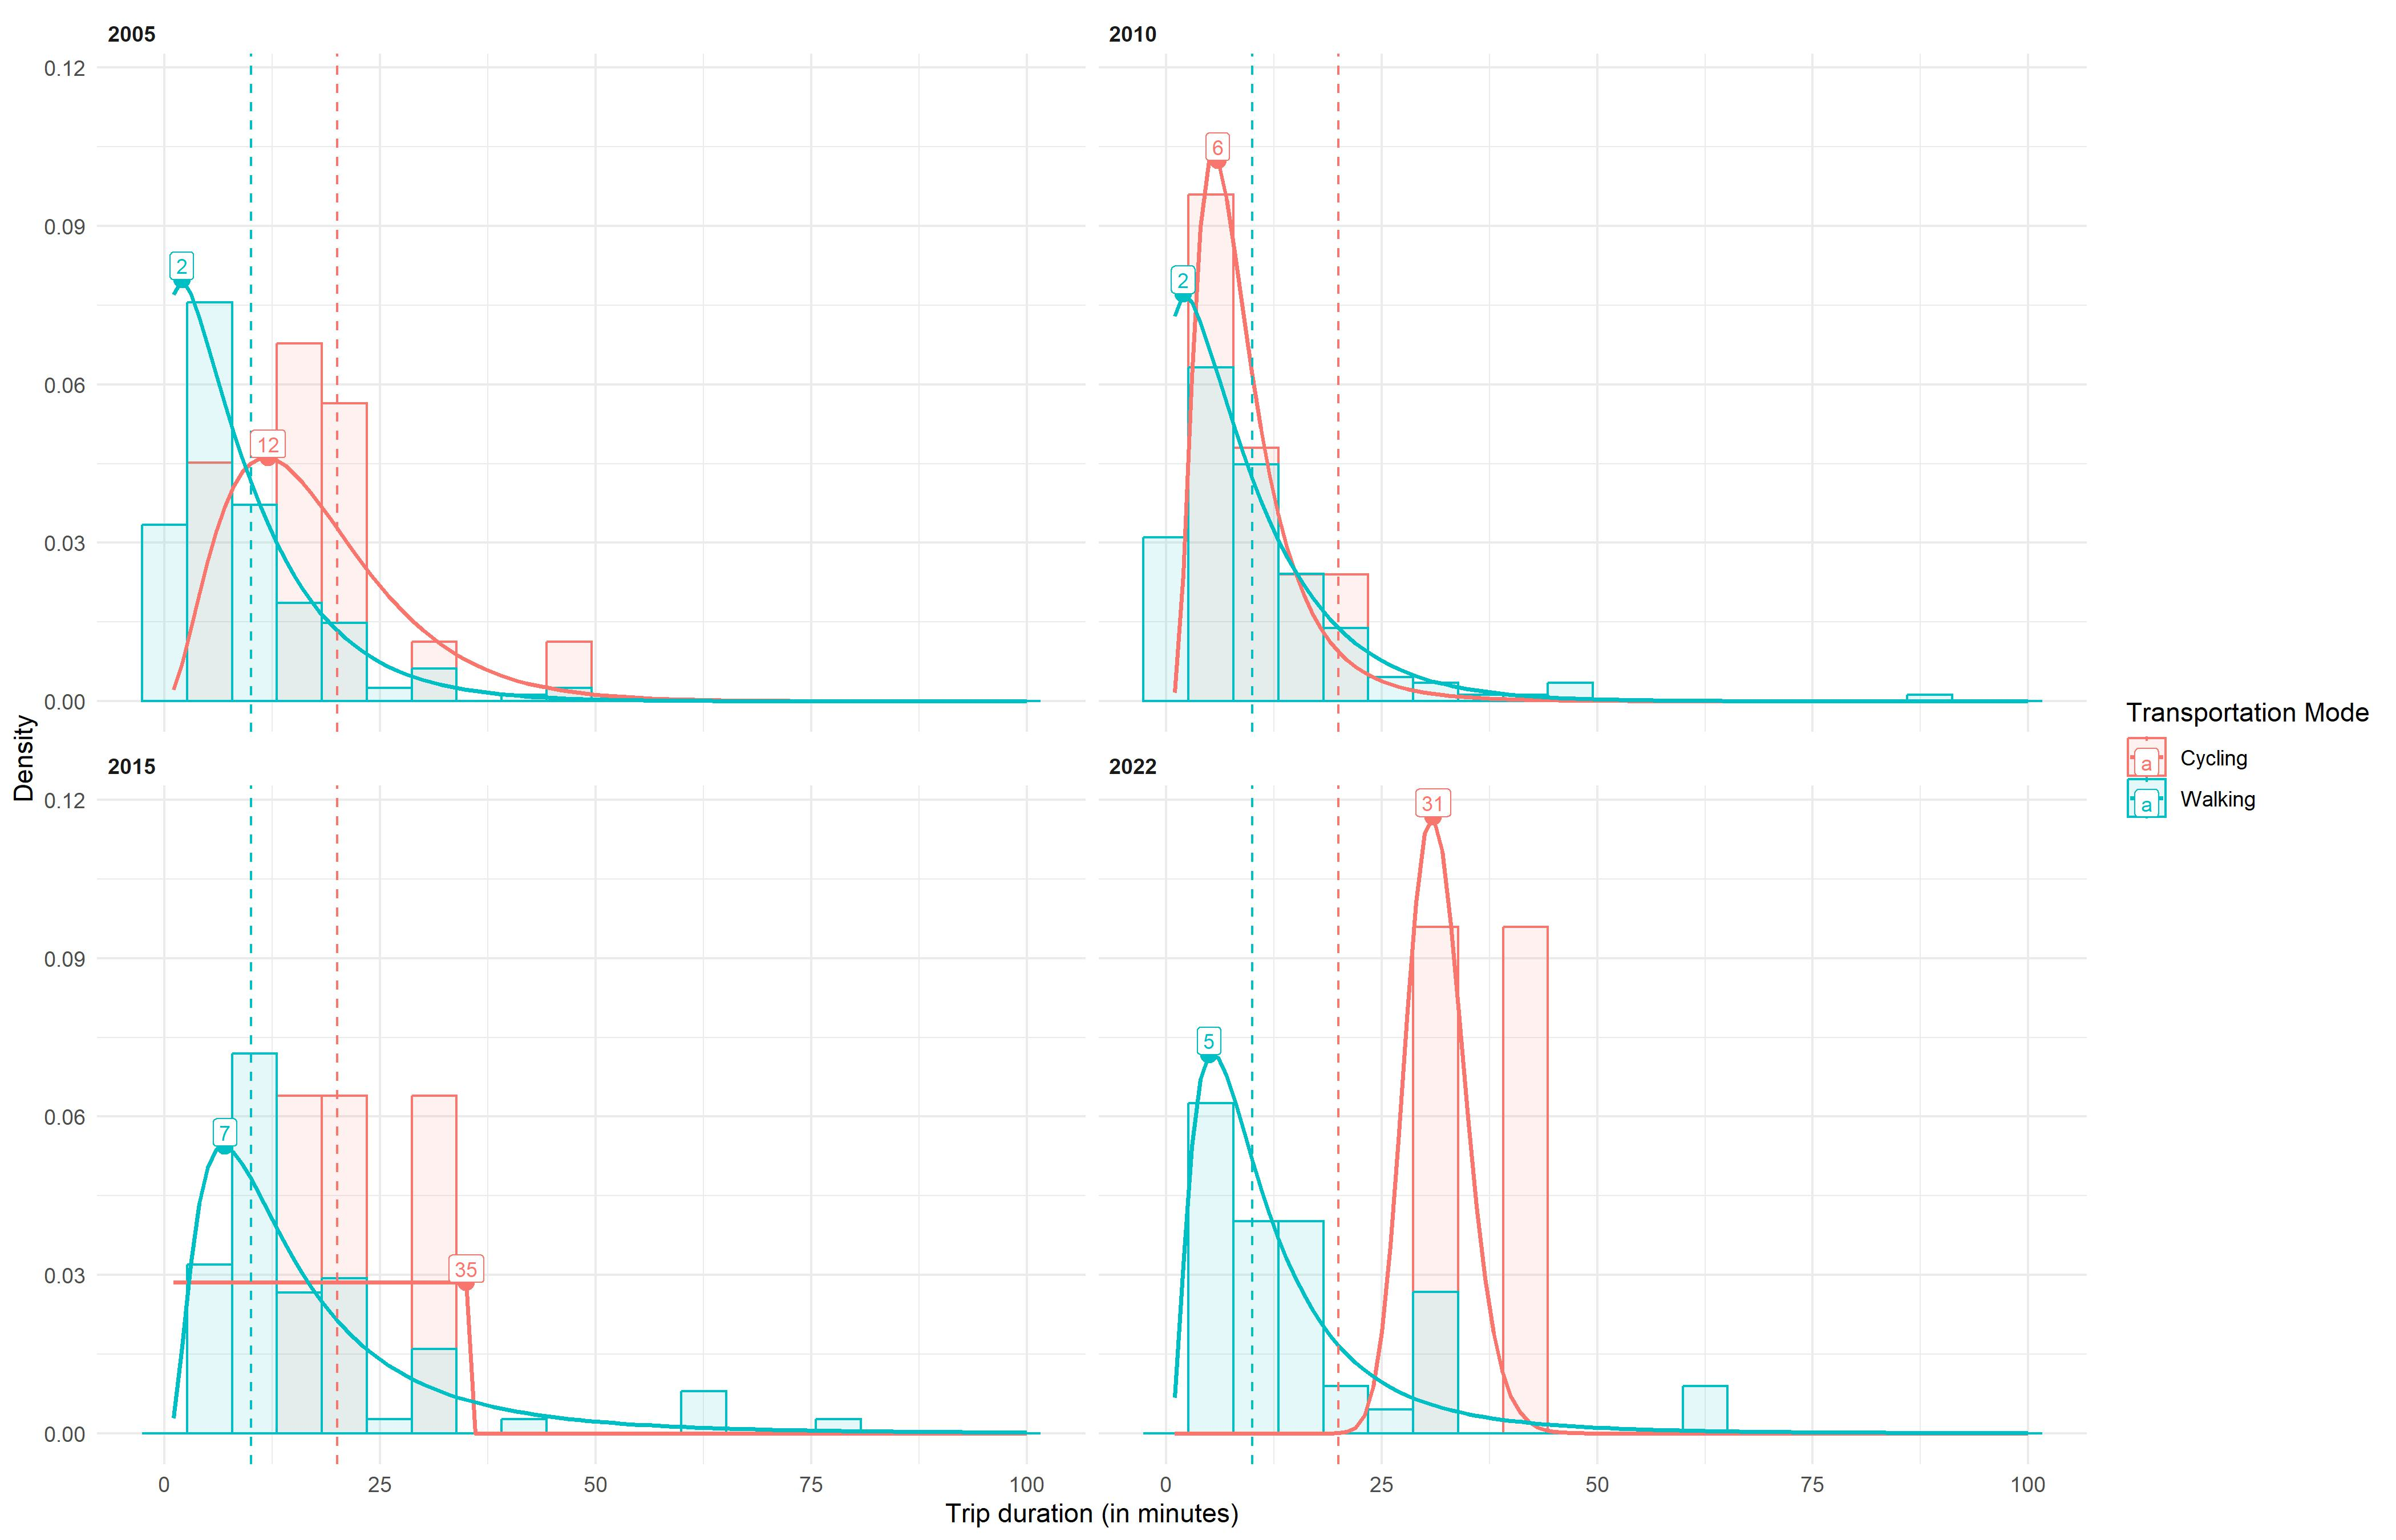
\includegraphics[width=1\linewidth]{figures/impf_Outdoors} 

}

\caption{Empirical data and impedance functions fitted for walking trips with `work or school` as destination.}\label{fig:outdoors-impedance-fig}
\end{figure}

For the years 2005 and 2010, the selected impedance functions are of the
gamma type, with shapes of \(\alpha = 1.24\) and \(\alpha = 1.27\),
respectively, and the same rate of \(\sigma = 0.13\). The rate parameter
(\(\sigma\)) mainly controls the speed of the curved drop, which is the
same for both years. The shape parameter (\(\mu\)) controls how the
density peak shifts in relation to the \(x\)-axis (the travel time). A
larger shape value means that the probability peak occurs at larger
values of time. Since the shape values for 2005 and 2010 are very close,
the peak of the PDF curve in both cases occurs at 2 minutes. Although
the difference in shape (\(\mu\)) between the two years is small and
does not change the time at which the peak occurs, it is enough to cause
a difference in the peak values themselves. In 2005, the walking trips
had a higher density around 2 minutes (0.079) compared to 2010 (0.077).

For 2015 and 2022, the PDFs that best represent the population's
transport behavior are lognormal distributions, with a mean of
\(\mu = 2.54\) and a standard deviation of \(\sigma = 0.79\) for 2015,
and a mean of \(\mu = 2.27\) and a standard deviation of
\(\sigma = 0.77\) for 2022. In 2015, the density peak (0.05) occurs at a
journey duration of 7 minutes. Here, we observe that a lower density
peak corresponds to a more dispersed curve, with higher densities at
longer durations. In fact, while in 2005 and 2010 walking trips had
densities close to zero for durations over 50 minutes, in 2015 there is
still a small density (0.002) at the 50-minute mark. In 2022, the
density peak (0.07) occurs at a duration of 5 minutes, and the curve is
less dispersed than in 2015, registering lower densities near the
50-minute mark (0.01), in comparison.

For trips made by bicycle, the best-fitting impedance function in 2005
is of the gamma type. For 2010 and 2022, the impedance functions are
best represented by lognormal distributions. In 2015, the PDF that best
fits the data is a uniform distribution, with an upper bound of 35
minutes and a peak density of 0.028. The presence of uniform functions
means that it was not possible to parameterize more complex functions
(like the other functions) and is explained by the low number of
episodes in this category of destination, mode of transport and year (in
this case, there were only 3 episodes identified). Overall, all the
uniform functions have a maximum of 6 episodes and all of them are for
the transportation mode cycling - which can be explained since this mode
of transport does not have many episodes compared to the walking
episodes (only 7\% of active travel episodes). The figure also shows how
cycling trips tend to have greater dispersion and higher typical values
(dashed vertical lines) when compared to walking trips.

The complexity of the impedance function depends on the number of
episodes available for calibration. For instance, fitting a gamma-type
function required an average of 219 episodes, while fitting a lognormal
function required approximately 176 episodes. In contrast, fitting a
normal function required only 5 episodes, and fitting a uniform function
required, on average, just 4 episodes.

The temporal difference between the decay functions is also evident in
Figure \ref{fig:walking-evolution-fig}, which shows the calibrated
functions for each year of analysis across all destination and transport
mode categories for walking trips. For some locations, the impedance
functions are of the same type and have similar parameters across all
the years analyzed. For example, the ``Cultural venues'', consistently
uses a gamma function to represent the population's transport behavior
for all the years analyzed. On the other hand, the ``Place of worship''
destination exhibits temporal differences, with distinctly different
peaks and density dispersions, reflecting the variations in the
empirical data shown in Figure \ref{fig:figure-boxplot} and discussed
above.

\begin{figure}

{\centering 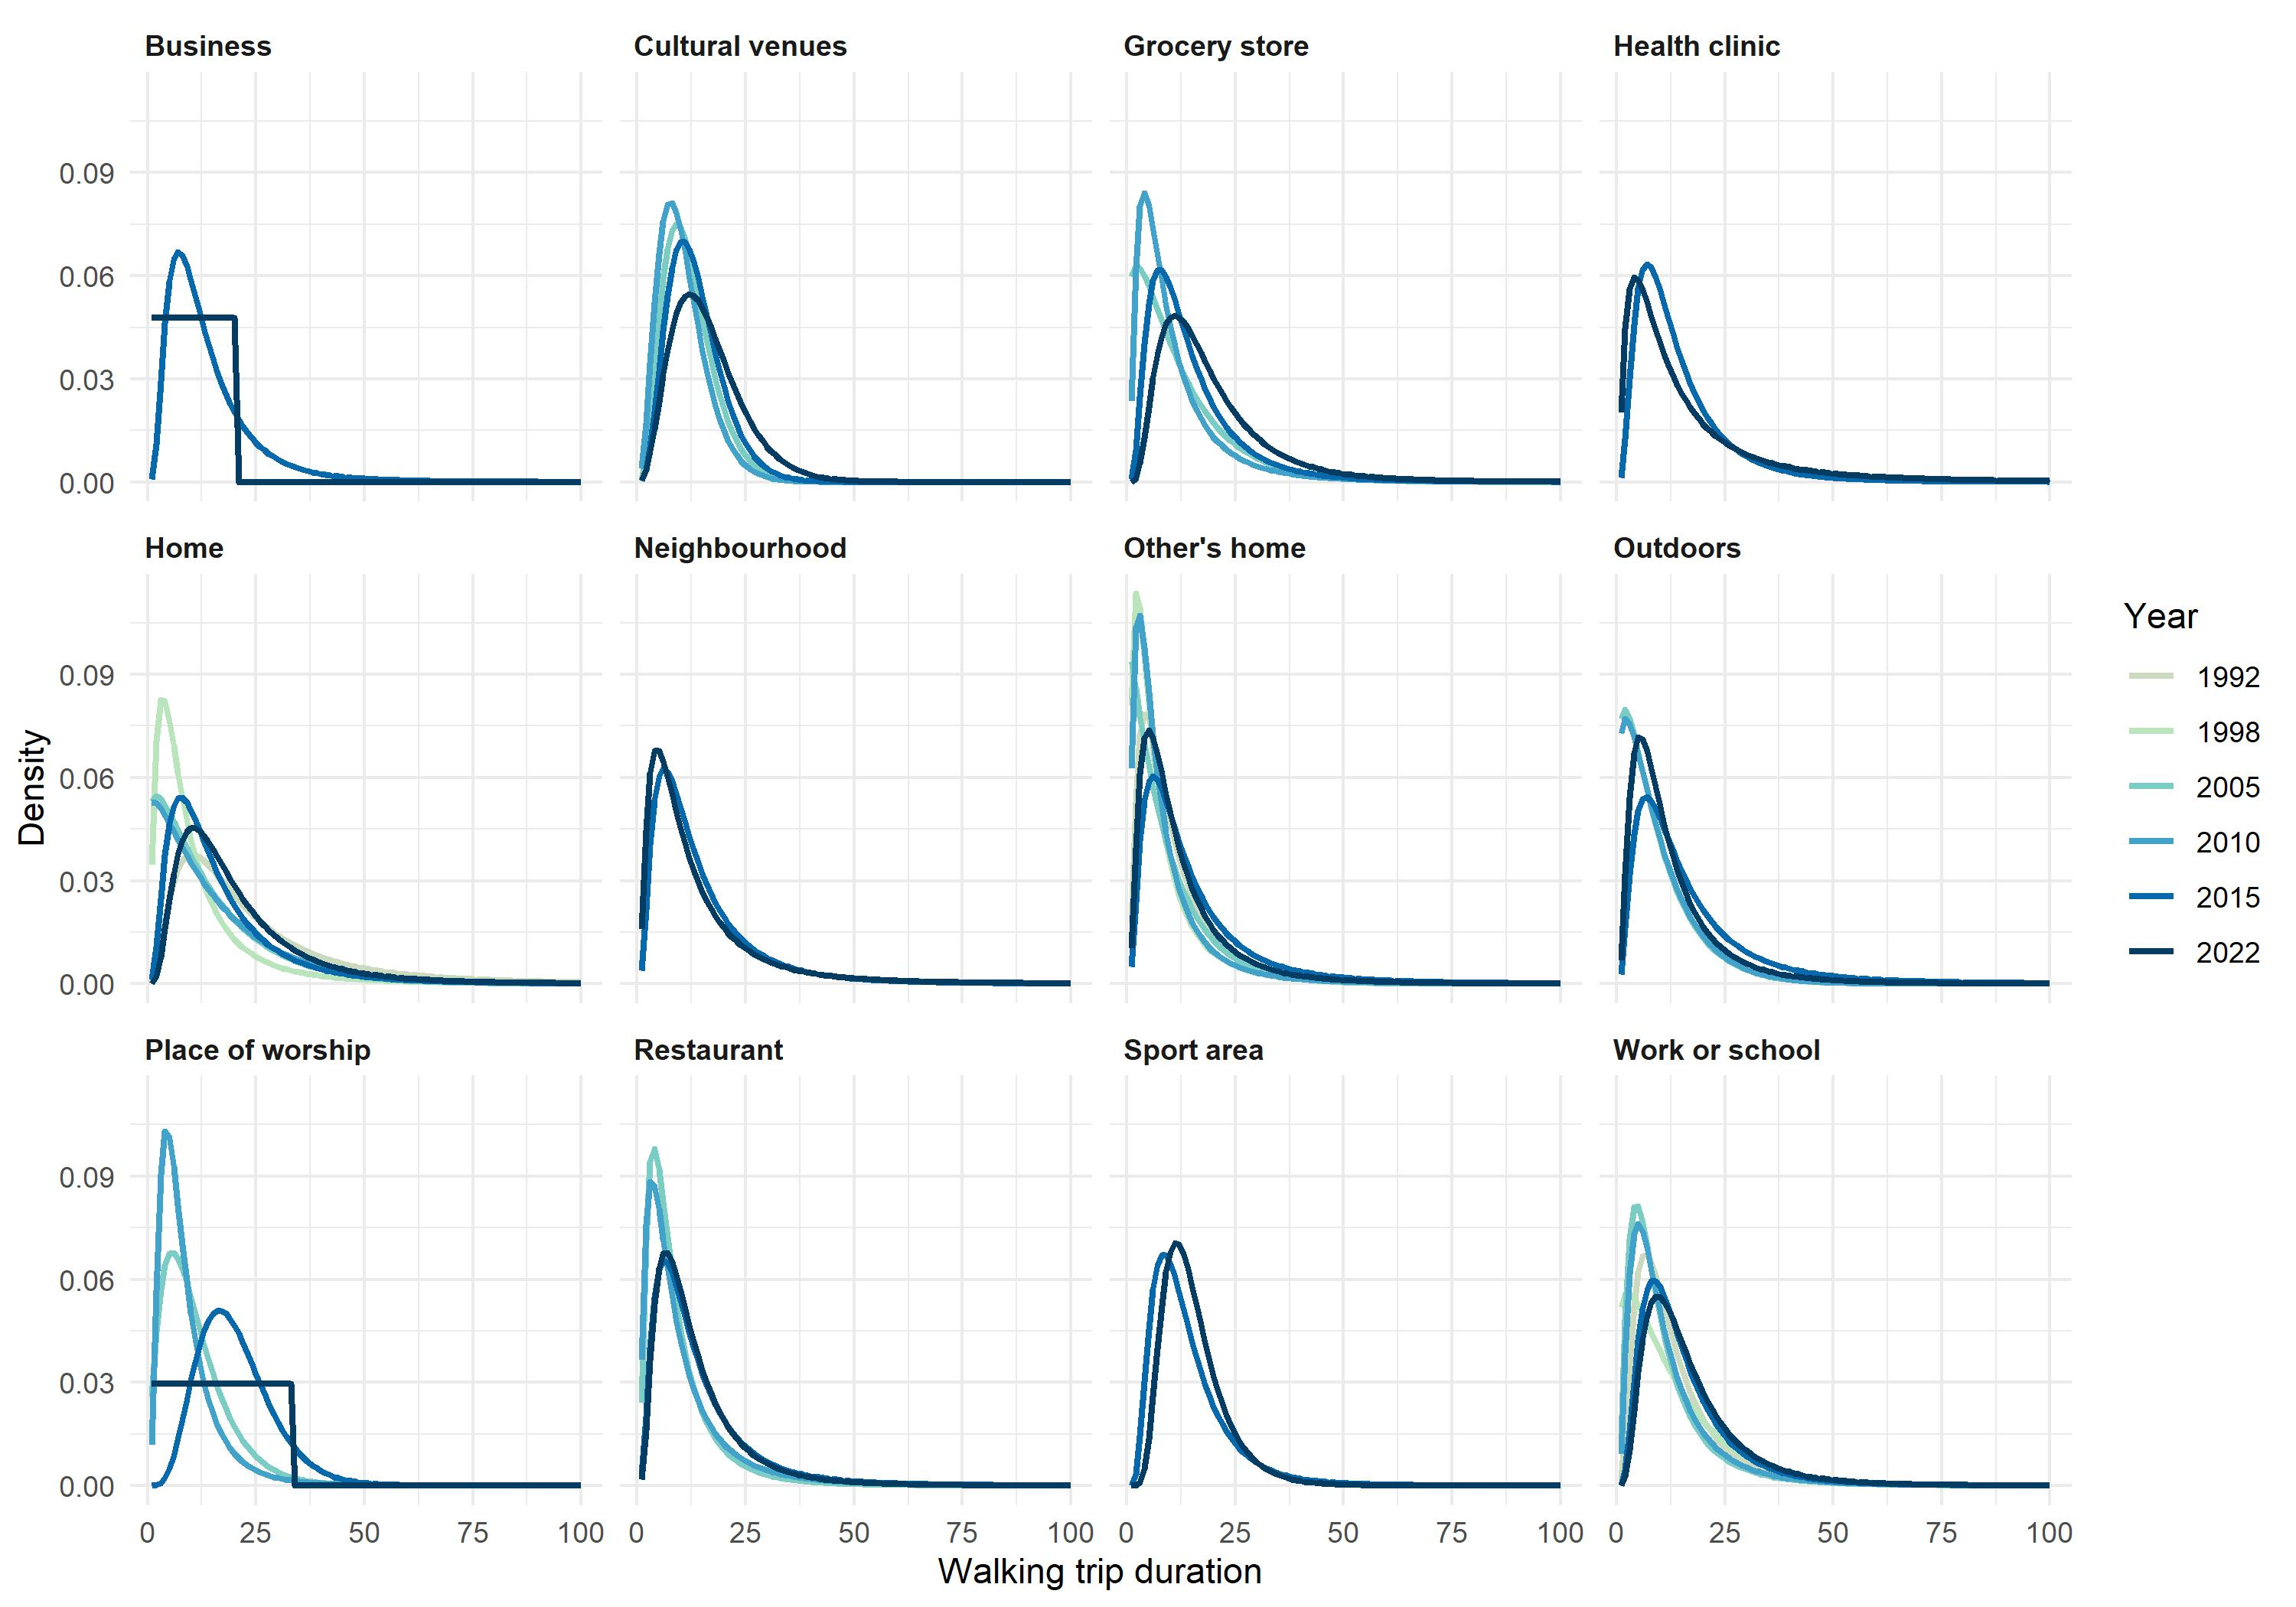
\includegraphics[width=1\linewidth]{figures/walking_temporal_evolution} 

}

\caption{Temporal evolution of walking impedance functions.}\label{fig:walking-evolution-fig}
\end{figure}

Finally, Figures \ref{fig:walking-function-by-year-fig} and
\ref{fig:cycling-function-by-year-fig} present the impedance functions
for different destination categories, grouped by year, for the walking
and cycling modes of transport, respectively.

\begin{figure}

{\centering 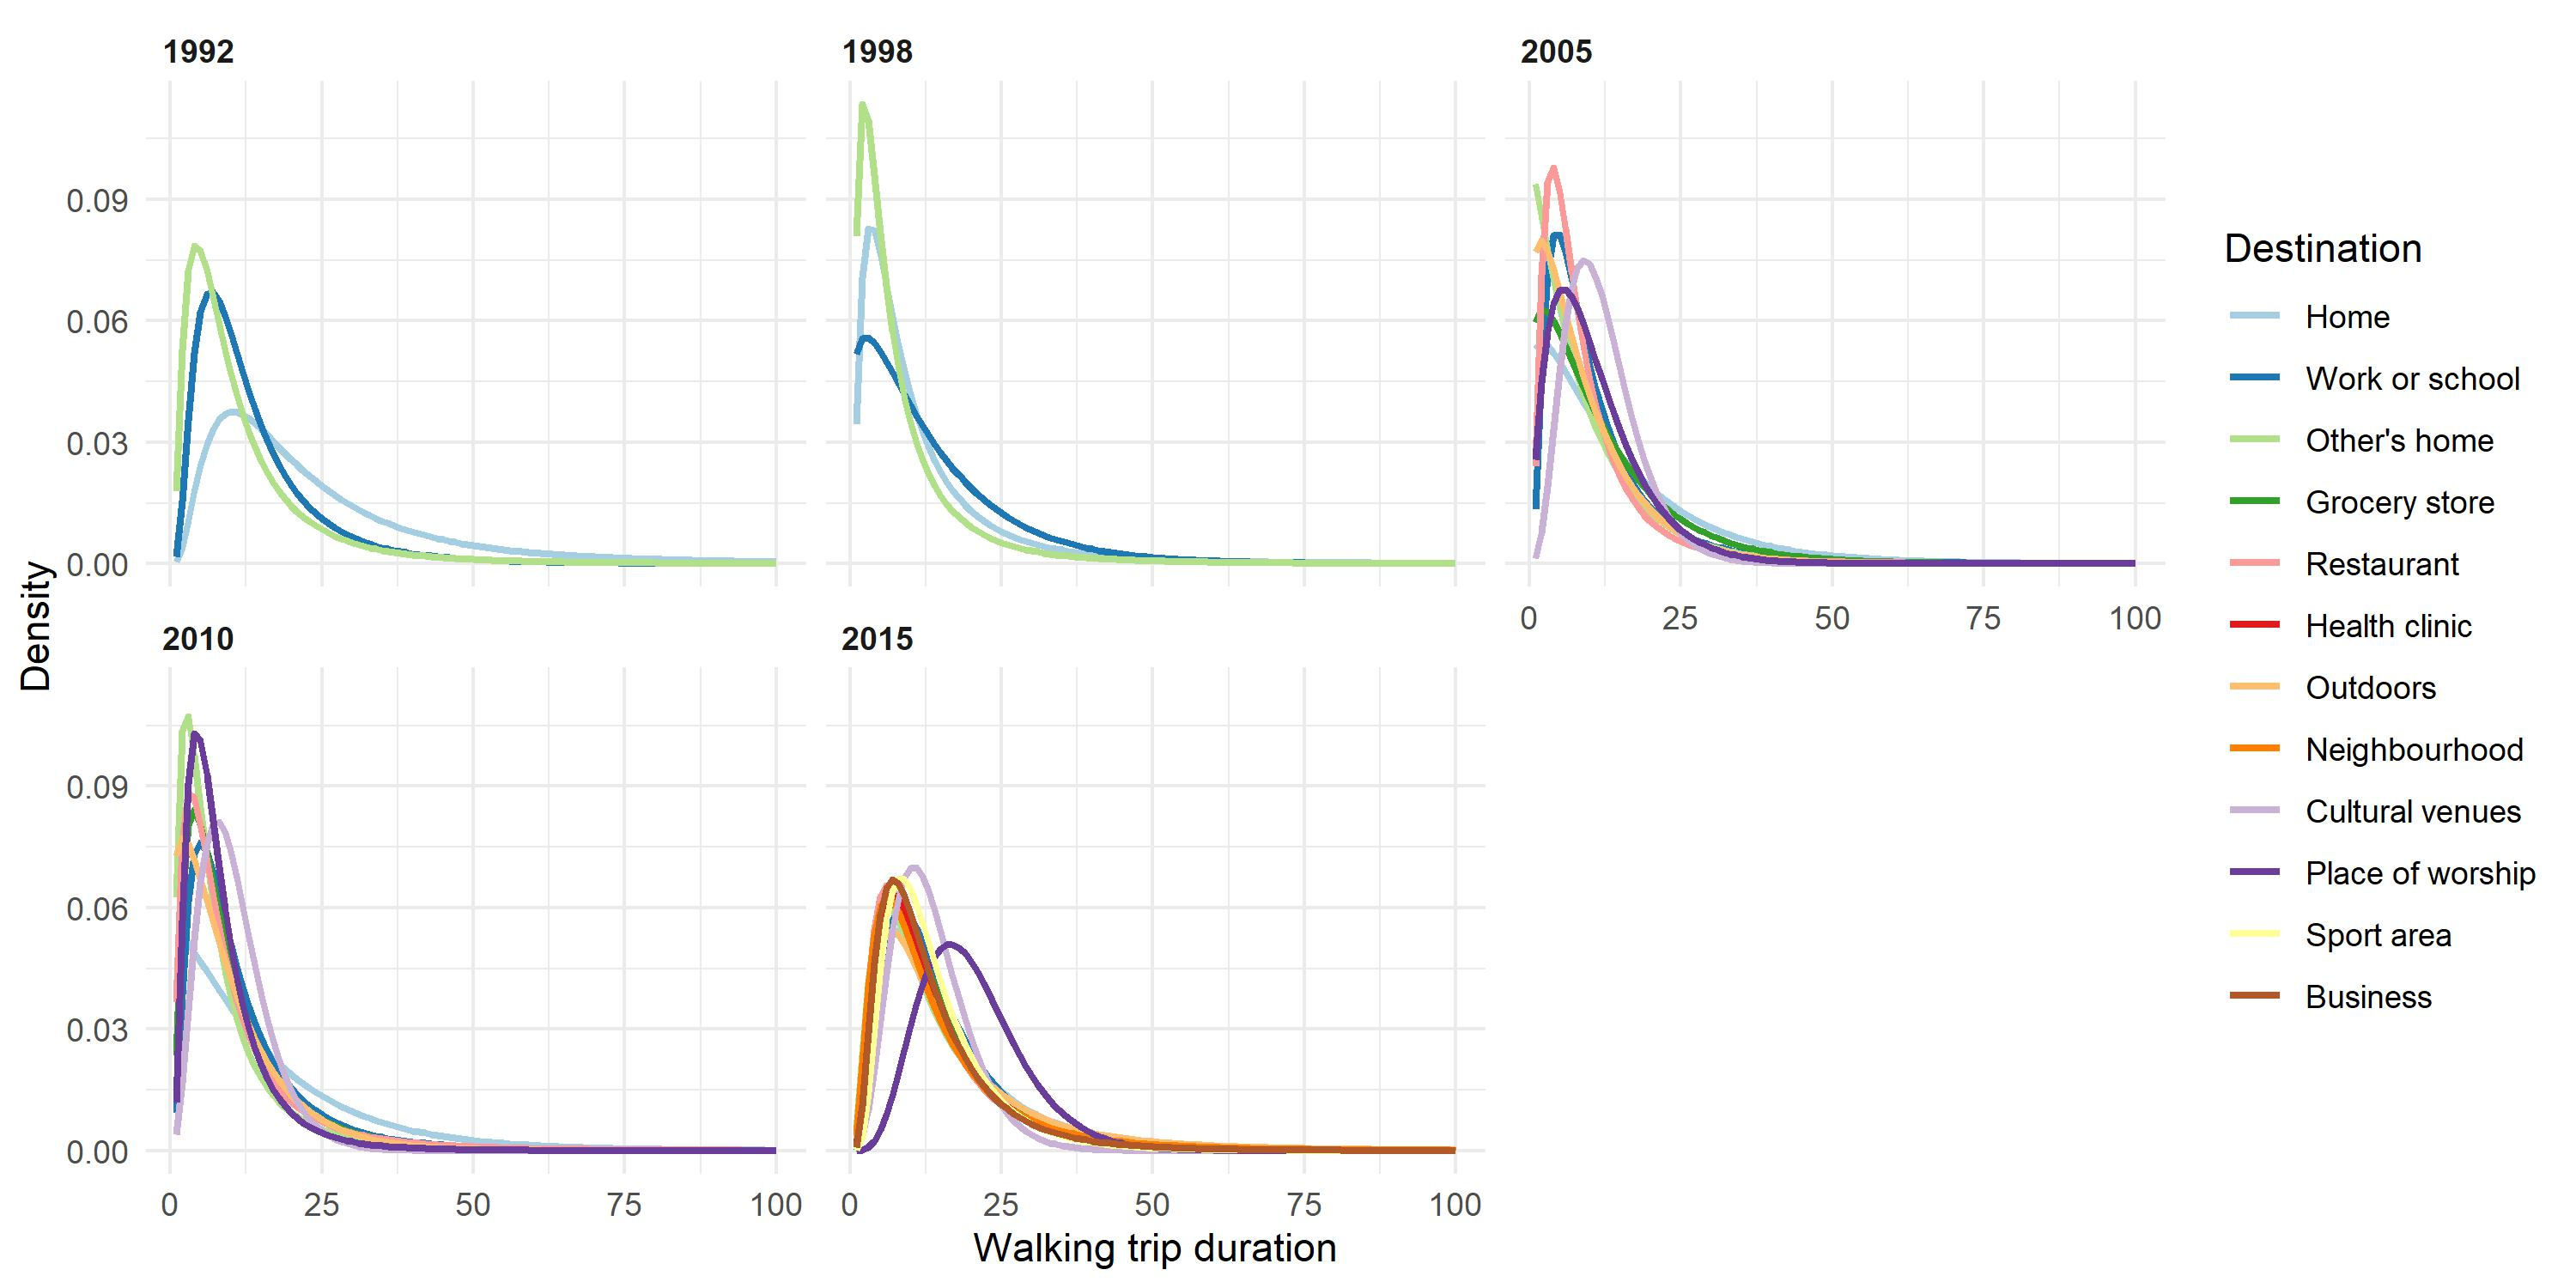
\includegraphics[width=1\linewidth]{figures/walking_functions_by_year} 

}

\caption{Walking functions grouped by year.}\label{fig:walking-function-by-year-fig}
\end{figure}

\begin{figure}

{\centering 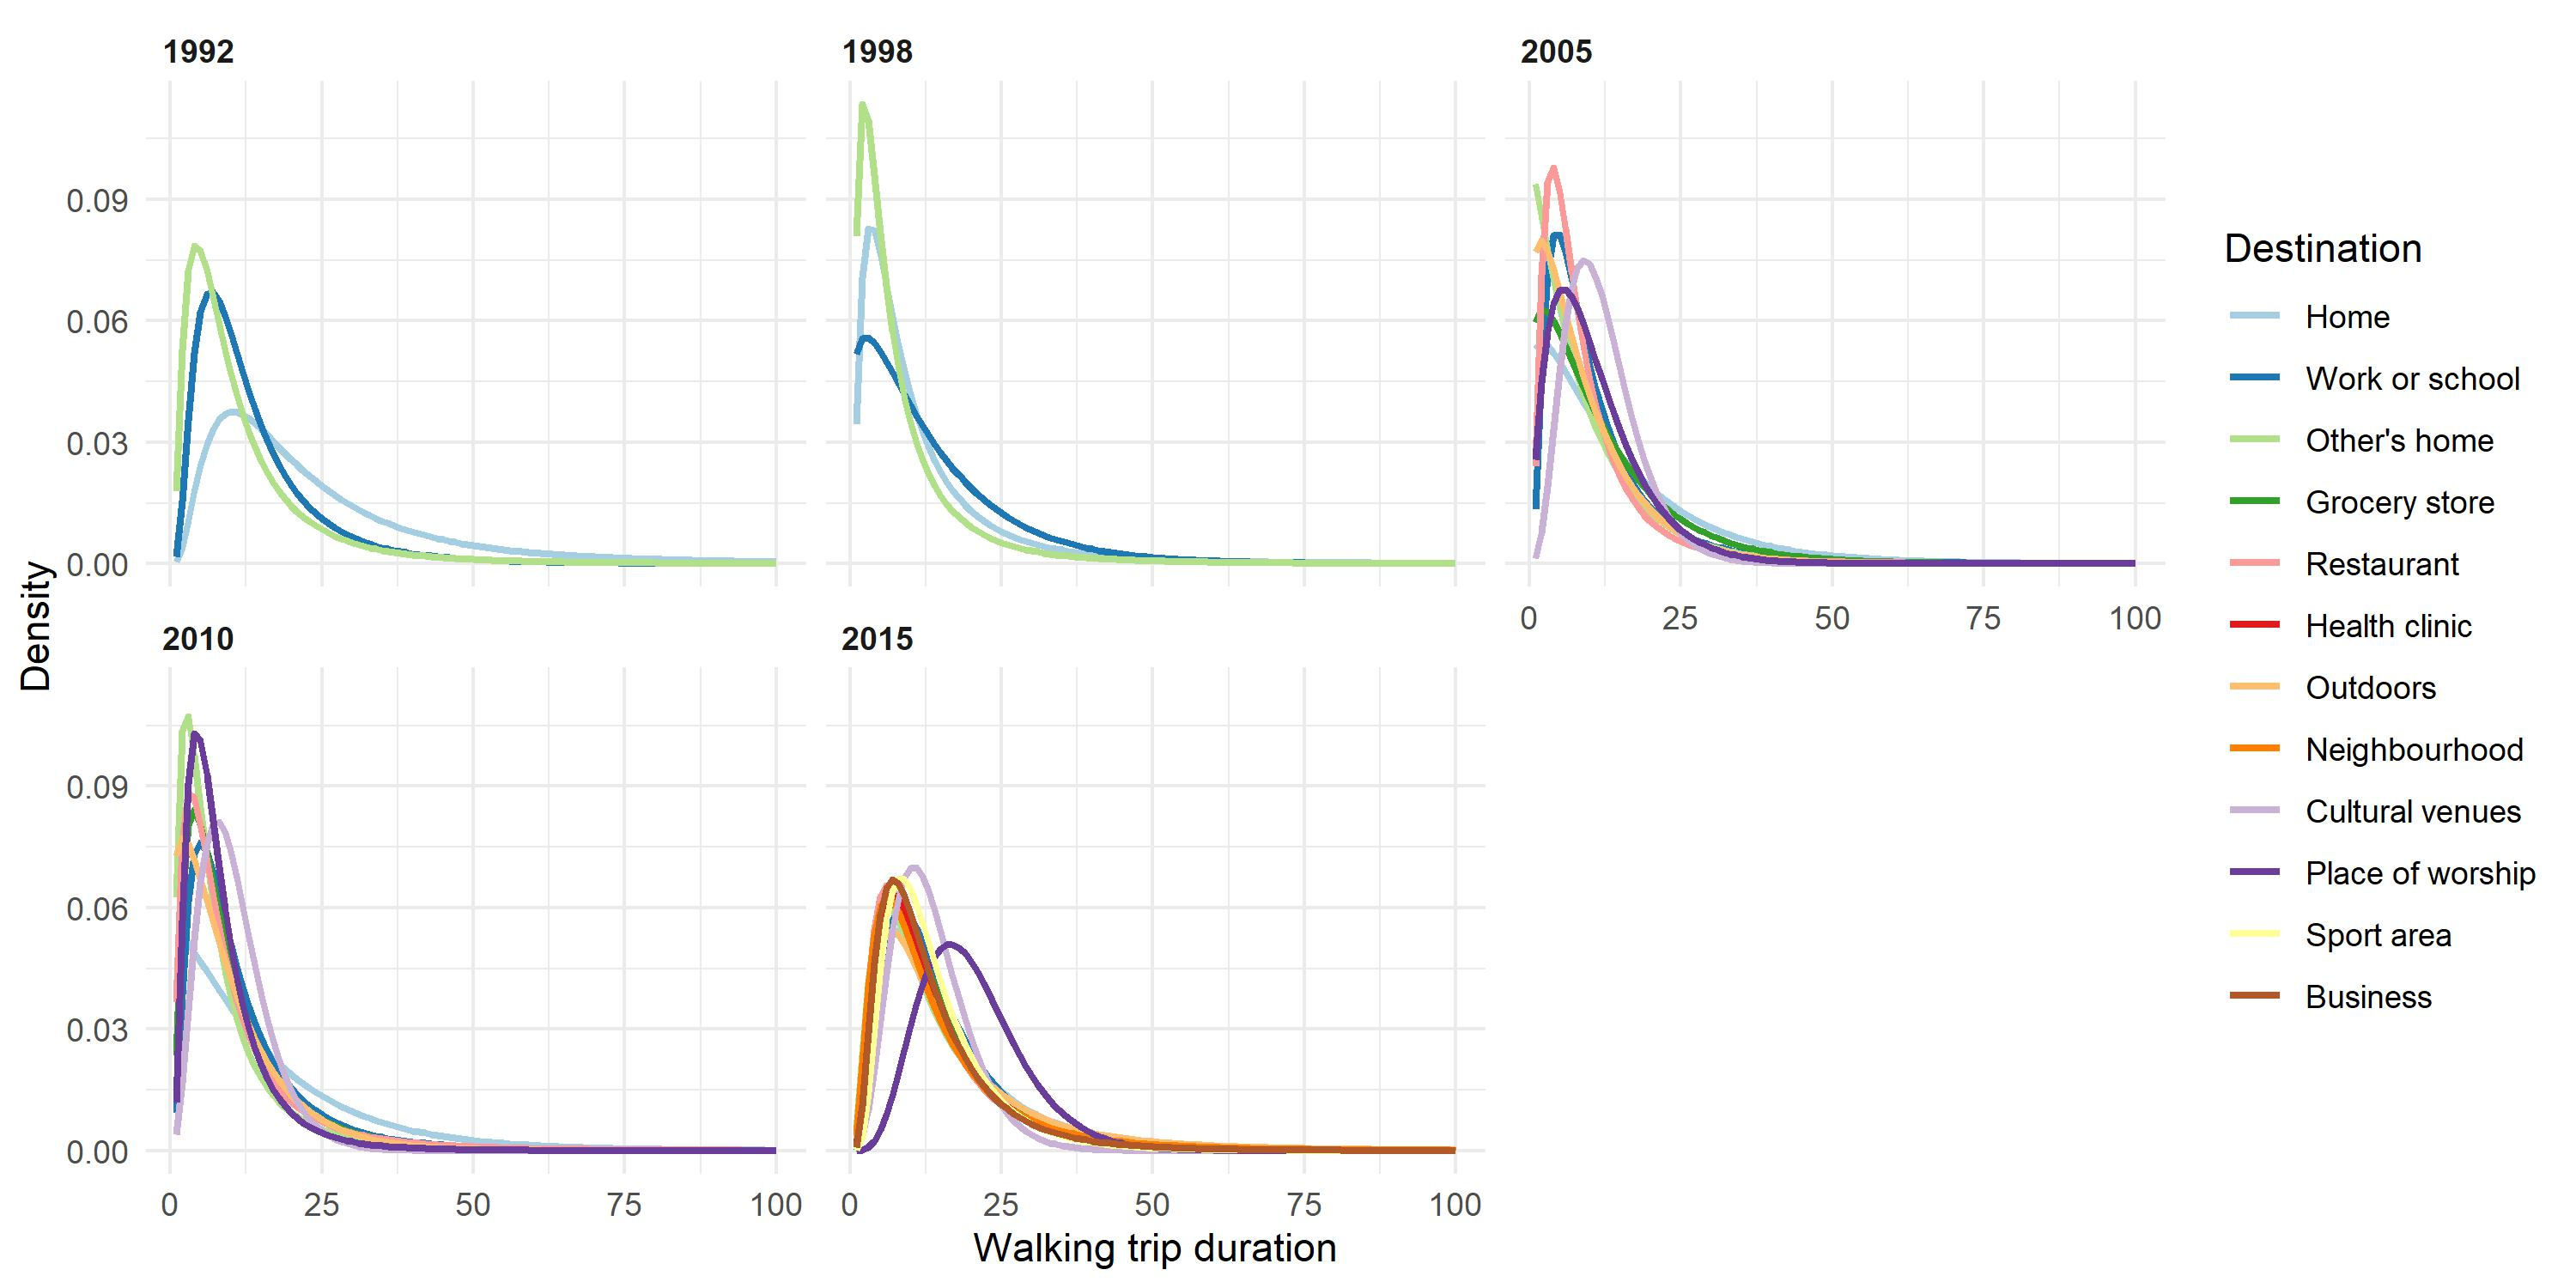
\includegraphics[width=1\linewidth]{figures/cycling_functions_by_year} 

}

\caption{Cycling functions grouped by year.}\label{fig:cycling-function-by-year-fig}
\end{figure}

\section{Summary and conclusion}\label{summary-and-conclusion}

The main objectives of this study were to provide an overview of active
transportation in Canadian metropolitan cities, focusing on primary
origins, destinations, and travel times, and to identify appropriate
impedance functions for active transportation modes across various
destinations and time periods. In this study we perform a direct
application of \texttt{ActiveCA} R package
\citep{dossantos2024ActiveCA}, analyzing over 12,000 cases of active
travel trips that represented 28,066,620 episodes, from the Time Use
cycles of the General Social Survey (GSS) from 1992 to 2015, covering a
twelve different type of destinations and considering walking and
cycling as transportation modes.

Although the study does not explain the reasons for fluctuations in
travel times over the years, the findings confirmed with statistical
significance, that typical active travel times remained constant for
walking mode, and increased after a dropped since 1998 for cycling mode.
For walking trips, typical travel times remained constant at 10 minutes
since 2005. For cycling trips, the typical travel time fluctuated from
20 minutes in 1992 to 25 minutes in 1998, dropped to 15 minutes in 2005,
dropped again to 10 minutes in 2010, and returned to increase to 20
minutes in 2015. The results also show that, in general, typical travel
times for walking were consistently lower than for cycling.

For walking trips, travel times to `Restaurants' and `Outdoors' rose
from 5 minutes in 2005 to 10 minutes in 2015, while travel to `Places of
worship' increased from 10 minutes in 2005 to 20 minutes in 2015,
marking the highest typical travel time for walking trips. The walking
travel time for `Home' and `Work or school' remained constant at 10
minutes since at least the three last GSS cycles. For cycling trips, the
year of 2015 displayed a trend of increasing travel times for almost all
destinations. This trend is perceptible and statistically significant
for `Grocery store' (rising from 10 to 15 minutes between 2005 and
2015), `Outdoors' (from 15 to 30 minutes during the same period), and
`Restaurant' (from 15 minutes in 2005 to 20 minutes in 2015). `Home'
returned to 20 minutes in 2015 after a drop to 10 minutes in 2010.

For both transportation modes, the destination `Other's home' showed a
decline in the share of trips, reflecting changes in travel behavior
since the technological advances enabled people to maintain contact with
friends and relatives without visiting in person. For walking trips,
findings indicate that `Home' remains the main hub, whether as an origin
or destination. For cycling trips, the combination of `Home' and `Work
or school' accounted for the largest share of trips.

The population share with at least one active trip record ranged from
7.8\% in 1998 (the lowest, 1,892,299 people) to 14.5\% in 2010 (the
peak, 4,084,114 people). In the most recent GSS survey, from 2015,
participation decreased to 11\% (3,265,846 people). Walking trips
dominate active trips. Approximately 84\% of the walking population and
90\% of the cycling population recorded only one trip. The maximum
number of trips recorded by a person was 10 (in 1992, 2005, and 2010)
for the walking population and 4 (in 2005) for the cycling population.
The number of active trips per person in the general population was
close to 0. Among the active population, this value averaged 1.180 trips
per person. A decreasing trend in the number of active episodes per
person was detected, whether analyzed in terms of walking or cycling
episodes.

The study highlights the need to apply specific impedance functions for
different destinations when measuring the cost decay effect in
accessibility analyses. Based on this, we fitted 64 impedance functions
for active transportation over more than 30 years, considering different
types of destinations and transportation modes. The results indicate
that none of the parameterized functions were exponential, suggesting
that the impedance functions commonly used in active accessibility
studies may not accurately capture travel behavior, especially for very
short trips (up to 3 minutes), by giving to shorter trips higher
probability of being made. Destinations with a high number of episodes
were primarily fitted with gamma functions, followed by lognormal
functions, while destinations with fewer episodes (fewer than six) were
fitted with a uniform distribution.

Given similarities in urbanization processes between Canada, the United
States, Australia, and West Europe, these findings may also be
applicable to metropolitan areas in those regions. Finally, this study
contributes to the ongoing discussion on active transportation,
emphasizing its importance in promoting sustainable transportation
planning.

\renewcommand\refname{References}
\bibliography{mybibfile.bib}


\end{document}
